\documentclass[a4paper]{book}
\usepackage{tocbibind} % for toc show inside pdf
\usepackage[
	%urlbordercolor = {1 1 1},
	%linkbordercolor = {1 1 1},
	%citebordercolor = {1 1 1},
    bookmarksnumbered, % add bookmark number in pdf output
	urlcolor = blue,
	colorlinks = true,
	citecolor = black,
	linkcolor = black]{hyperref}
\usepackage{graphicx}
\usepackage{xltxtra}
\usepackage{fancyhdr}
\usepackage{booktabs}
\usepackage{indentfirst}
\usepackage{framed,color}
\usepackage{footnpag}
\usepackage{listings}
\usepackage{array}
\usepackage[font=small,format=plain,labelfont=bf,up,textfont=it,up]{caption}

\usepackage{titlesec} % texlive-latex-extra package
\usepackage[titletoc]{appendix} % this is used for \appendices

\usepackage[usenames,dvipsnames]{xcolor}

\definecolor{colorchapter}{RGB}{70,130,180}     % SteelBlue
\definecolor{colorsection}{RGB}{95,158,160}    % CadetBlue
\definecolor{colorsubsection}{RGB}{139,0,0} % DarkRed
\definecolor{colorheader}{RGB}{70,130,180} % SteelBlue

\definecolor{mygreen}{rgb}{0,0.6,0}
\definecolor{mygray}{rgb}{0.5,0.5,0.5}
\definecolor{mymauve}{rgb}{0.58,0,0.82}
\definecolor{CPPViolet}{HTML}{7040A0}

\lstset{
    backgroundcolor = \color[RGB]{245,245,244},
    basicstyle = \footnotesize,
    breakatwhitespace = false,
    breaklines = true,       
    captionpos = b,                    
    commentstyle = \color{mygreen}\bfseries,
    extendedchars = false,             
    frame = shadowbox,
    framerule = 0.5pt,
    keepspaces = true,
    keywordstyle = \color{blue}\bfseries,     % keyword style
    language = C++, % the language of code
    otherkeywords = {string}, 
    numbers = left, 
    numbersep = 5pt,
    numberstyle = \footnotesize\color{darkgray},
    rulecolor = \color{black}, 
    showspaces = false, 
    showstringspaces = false, 
    showtabs = false,
    stepnumber = 1,         
    stringstyle = \color{mymauve},    % string literal style
    tabsize = 2,          
    title = \lstname
    morekeywords = {alignas,continute,friend,register,true,alignof,decltype,goto,
    reinterpret_cast,try,asm,defult,if,return,typedef,auto,delete,inline,short,
    typeid,bool,do,int,signed,typename,break,double,long,sizeof,union,case,
    dynamic_cast,mutable,static,unsigned,catch,else,namespace,static_assert,using,
    char,enum,new,static_cast,virtual,char16_t,char32_t,explict,noexcept,struct,
    void,export,nullptr,switch,volatile,class,extern,operator,template,wchar_t,
    const,false,private,this,while,constexpr,float,protected,thread_local,
    const_cast,for,public,throw,std}, 
    emph = {map,set,multimap,multiset,unordered_map,unordered_set,
    unordered_multiset,unordered_multimap,vector,string,list,deque,
    array,stack,forwared_list,iostream,memory,shared_ptr,unique_ptr,
    random,bitset,ostream,istream,cout,cin,endl,move,default_random_engine,
    uniform_int_distribution,iterator,algorithm,functional,bing,numeric,},
    emphstyle = \color{CPPViolet},               
}


\titleformat{\section}
{\color{colorsection}\normalfont\Large\bfseries}
{\color{colorsection}\thesection}{1em}{}
\titleformat{\subsection}
{\color{colorsubsection}\normalfont\large\bfseries}
{\color{colorsubsection}\thesubsection}{1em}{}

\definecolor{shadecolor}{gray}{0.90}

\setromanfont[Mapping=tex-text,BoldFont=WenQuanYi Micro Hei]{AR PL SungtiL GB}
\setmonofont{WenQuanYi Zen Hei Mono}
{\setmainfont{Courier New Bold}

\XeTeXlinebreaklocale{zh}
\XeTeXlinebreakskip=0em plus 0.1em minus 0.01em
\XeTeXlinebreakpenalty=0

\settowidth{\parindent}{文文}
\setcounter{footnote}{0}

\title{{OMNeT++入门指南}}
\author{Zackary Wang}

\makeatletter
\let\savedauthor=\@author
\let\savedtitle=\@title
\def\imgwidth{.6\linewidth}
\def\maxwidth{\ifdim\Gin@nat@width>\imgwidth\imgwidth
\else\Gin@nat@width\fi}
\makeatother

\title{\huge{\savedtitle}}

\author{\textbf{\savedauthor}\thanks{This is the PDF file for the Agile Software Development book contents. It is licensed under the Creative Commons Attribution-Non Commercial-Share Alike 3.0 license. I hope you enjoy it, I hope it helps you learn the software development, and I hope you'll continuously watch this : \url{http://github.com/larrycai/sdcamp}, will be happy if you follow my weibo \url{http://weibo.com/larrycaiyu}}}
\def\w3cdtfymd{\the\year-\ifnum\month<10 0\fi\the\month-\ifnum\day<10 0\fi\the\day}
\date{\w3cdtfymd}
%\renewcommand{\thefootnote}{\fnsymbol{footnote}}

\newcommand{\PreserveBackslash}[1]{\let\temp=\\#1\let\\=\temp}
\let\PBS=\PreserveBackslash
\makeatletter
  \setlength\headheight{12\p@}
  \setlength\headsep   {.25in}
  \setlength\topskip   {10\p@}
  \setlength\footskip{.35in}
  \setlength\textwidth{400\p@}
  
  \setlength\@tempdima{\paperheight}
  \addtolength\@tempdima{-2in}
  \divide\@tempdima\baselineskip
  \@tempcnta=\@tempdima
  \setlength\textheight{\@tempcnta\baselineskip}
  \addtolength\textheight{\topskip}
  
  \setlength\@tempdima        {\paperwidth}
  \addtolength\@tempdima      {-\textwidth}
  \setlength\oddsidemargin    {\paperwidth}
  \addtolength\oddsidemargin  {-2.35in}
  \addtolength\oddsidemargin  {-\textwidth}
  \setlength\marginparwidth   {0pt}
  \@settopoint\oddsidemargin
  \@settopoint\marginparwidth
  \setlength\evensidemargin  {\paperwidth}
  \addtolength\evensidemargin{-2.35in}
  \addtolength\evensidemargin{-\textwidth}
  \@settopoint\evensidemargin
  
  \setlength\topmargin{\paperheight}
  \addtolength\topmargin{-2in}
  \addtolength\topmargin{-\headheight}
  \addtolength\topmargin{-\headsep}
  \addtolength\topmargin{-\textheight}
  \addtolength\topmargin{-\footskip}     % this might be wrong!
  \addtolength\topmargin{-.5\topmargin}
  \@settopoint\topmargin
  %\@addtoreset{footnote}{page}  
\makeatother

%\fancypagestyle{plain}{\fancyhf{}\fancyfoot[LE,RO]{\footnotesize\textbf\thepage}}
\fancypagestyle{plain}{\fancyhf{}\fancyfoot{}} % make sure no page number in page of first chapter

\pagestyle{plain}


\renewcommand{\headrulewidth}{0pt}
\renewcommand{\footrulewidth}{0pt}

\newcounter{img}[chapter]
\renewcommand{\theimg}{\thechapter.\arabic{img}}
\newcommand{\img}[1]{\begin{figure}[h!]
	\refstepcounter{img}
	\label{img:\theimg}
	\centering\includegraphics[width=\maxwidth]{figures/\theimg.png}
	\caption{#1}
\end{figure}}

% below for code syntax highlight
\usepackage{fancyvrb}
%\DefineShortVerb[commandchars=\\\{\}]{\|}
\DefineVerbatimEnvironment{Highlighting}{Verbatim}{commandchars=\\\{\},frame=leftline,fontsize=\small}
% Add ',fontsize=\small' for more characters per line
\newenvironment{Shaded}{}{}
\newcommand{\KeywordTok}[1]{\textcolor[rgb]{0.00,0.44,0.13}{\textbf{{#1}}}}
\newcommand{\DataTypeTok}[1]{\textcolor[rgb]{0.56,0.13,0.00}{{#1}}}
\newcommand{\DecValTok}[1]{\textcolor[rgb]{0.25,0.63,0.44}{{#1}}}
\newcommand{\BaseNTok}[1]{\textcolor[rgb]{0.25,0.63,0.44}{{#1}}}
\newcommand{\FloatTok}[1]{\textcolor[rgb]{0.25,0.63,0.44}{{#1}}}
\newcommand{\CharTok}[1]{\textcolor[rgb]{0.25,0.44,0.63}{{#1}}}
\newcommand{\StringTok}[1]{\textcolor[rgb]{0.25,0.44,0.63}{{#1}}}
\newcommand{\CommentTok}[1]{\textcolor[rgb]{0.38,0.63,0.69}{\textit{{#1}}}}
\newcommand{\OtherTok}[1]{\textcolor[rgb]{0.00,0.44,0.13}{{#1}}}
\newcommand{\AlertTok}[1]{\textcolor[rgb]{1.00,0.00,0.00}{\textbf{{#1}}}}
\newcommand{\FunctionTok}[1]{\textcolor[rgb]{0.02,0.16,0.49}{{#1}}}
\newcommand{\RegionMarkerTok}[1]{{#1}}
\newcommand{\ErrorTok}[1]{\textcolor[rgb]{1.00,0.00,0.00}{\textbf{{#1}}}}
\newcommand{\NormalTok}[1]{{#1}}
% end of code syntax highlight

\newcounter{tab}[chapter]
\renewcommand{\thetab}{\thechapter.\arabic{tab}}

\newcommand{\prechap}{第}
\newcommand{\postchap}{章}
\newcommand{\presect}{}
\newcommand{\postsect}{节}
\renewcommand{\chaptermark}[1]{\markboth{\textbf{\prechap \thechapter \postchap}\hspace*{1ex}#1}{}}
\renewcommand{\sectionmark}[1]{\markright{\textbf{\presect \thesection \postsect}\hspace*{1ex}#1}}
\newcommand{\chap}[1]{\newpage\thispagestyle{empty}\chapter{#1}\label{chap:\thechapter}}
\newcommand{\chapref}[1]{\hyperref[chap:#1]{\prechap #1\postchap}}
\newcommand{\imgref}[1]{\hyperref[img:#1]{图 #1}}
\newcommand{\tabref}[1]{\hyperref[tab:#1]{表 #1}}
\newcommand{\e}[1]{$ \times 10^{#1}$}
\renewcommand{\contentsname}{目录}
\renewcommand{\figurename}{图 }
\renewcommand{\tablename}{表 }
\renewcommand{\appendixname}{附录 }

% chapter 
\makeatletter
\def\@makechapterhead#1{%
  \vspace*{50\p@}%
  {\parindent \z@ \raggedright \normalfont
    \ifnum \c@secnumdepth >\m@ne
      \if@mainmatter
        \color{colorchapter}\normalfont\huge\bfseries\prechap{ }\thechapter{ }\postchap
        \par\nobreak
        \vskip 20\p@
      \fi
    \fi
    \interlinepenalty\@M
    \color{colorchapter}\normalfont\Huge\bfseries #1\par\nobreak
    \vskip 40\p@
  }}  
 
% this is for non-normal chapter like Acknownledgement, Preface, Contents  
\def\@makeschapterhead#1{%
  \vspace*{50\p@}%
  {\parindent \z@ \raggedright \normalfont
    \ifnum \c@secnumdepth >\m@ne
      \if@mainmatter
        \color{colorchapter}\normalfont\huge\bfseries \thechapter{ }
        \par\nobreak
        \vskip 20\p@
      \fi
    \fi
    \interlinepenalty\@M
    \color{colorchapter}\normalfont\Huge\bfseries #1\par\nobreak
    \vskip 40\p@
  }}  
\makeatother

\linespread{1.3}

\begin{document}
%\maketitle
% includes cover directly, pdf is generated from slides (could be word and others)

\includegraphics[scale=0.8]{img/cover.pdf}

\thispagestyle{empty}
\setcounter{tocdepth}{4}

\frontmatter
% preface
\&nbsp;
\&nbsp;
\&nbsp;

\&nbsp;
\&nbsp;



\&nbsp;

\&nbsp;

\&nbsp;

\&nbsp;

\&nbsp;

\&nbsp;

\&nbsp;

\&nbsp;

\&nbsp;





\&nbsp;

\&nbsp;

\&nbsp;

\&nbsp;

\&nbsp;

\&nbsp;

\tableofcontents\newpage\thispagestyle{empty}

% customize header & footer

\fancyhf{}
\fancyhead[LE]{\color{colorheader}\quad\small\textbf\thepage\quad\quad\small\leftmark}
\fancyhead[RO]{\color{colorheader}\small\rightmark\quad\quad\small\textbf\thepage\quad}
%\fancyhead[RE,LO]{\color{colorheader}\small{\savedtitle}} % book title 
%\fancyfoot[LE,RO]{\small\textbf\thepage} % page number
%\fancyfoot[C]{\small\textbf{hello}} % could add release information

%\renewcommand{\headrulewidth}{0.4pt}  % add one line
%\renewcommand{\headrule}{\color{red}} % conflict with headrulewidth
\pagestyle{fancy}

\mainmatter
%chapters
\chapter{OMNeT++仿真平台}
\label{omnet仿真平台}

\section{OMNeT++简介}
\label{omnet简介}

OMNeT++,一个基于Eclipse开发套件的开源网络仿真工具,目前主要在高校实验室进行一些网络仿真测试,对一些算法进行对比,它可以供使用者进行完成以下开发:

\begin{itemize}
\item \textbf{C\slash C++开发}

\item \textbf{网络仿真程序设计}

\end{itemize}

毫无疑问,基于Eclipse的开发工具肯定能支持普通的C\slash C++工程。
另外,在OMNeT++上网络仿真设计领域的优势在于,它是一个开源的项目,对大量的网络模型都提供代码支持。但是问题在于国内的确没有什么社区支持,出现问题只能自己解决,其实对于开源的项目大多存在这种问题,往往开源的项目,使用起来难度较大,开源项目往往比那些商业的软件开发难度较大,支持也较少,开源可不代表简单。

OMNeT++对初学者能力要求高,它假定使用者对编程有一定了解的,对eclipse开发环境也是特别熟悉的,另外这是一个网络仿真的软件,需要你对计算机网络有足够的认识,它提供了大量现有各种网络的仿真例子,如果你对网络认识足够强,那么这个软件你用起来会感到特别顺手。
目前有大量的开源仿真库用于OMNeT++环境,拥有丰富的外文资料,官方将其分为两类,包括Supported Models和Contributed Models:

\begin{itemize}
\item Supported Models

\end{itemize}

模型库的开发处于激活状态,有开发者在维护,定期会推出新的版本。

\begin{itemize}
\item Contributed Models

\end{itemize}

完成后只推出过一次或几次版本,目前没有人在维护。

\section{OMNeT++开源库}
\label{omnet开源库}

下面简单介绍一下几种常见的开源库。

\subsection{INET}
\label{inet}

由Simucraft公司主持开发,用于仿真有线及无线网络。

\begin{itemize}
\item 应用层协议:HTTP、FTP、Telnet、不同优先级的 Video、Ping;

\item 传输层协议:TCP、UDP、RTP ( RealtimeTransport Protocol );

\item 网络层协议:IPv4、IPv6、OSPF、AODV、DSDV、DSR等;

\item 数据链路层协议:Ethernet、PPP、IEEE 802.11、FDDI、Token Ring;

\item 官网:\href{http://inet.omnetpp.org}{http:\slash \slash inet.omnetpp.org}

\end{itemize}

\subsection{INETMANET}
\label{inetmanet}

由 Simucraft 公司主持开发,用于仿真无线、有线网络,在INET的基础上增加了大量的MANET协议,INETMANET=INET+MANET,在INET的基础上增加:

\begin{itemize}
\item 802.11a

\item Ieee80211Mesh,Ieee80211MeshMgmt

\item radiomodels: TwoRayModel, ShadowingModel, qamMode

\item Ns2MotionMobility

\item ARP:global ARP cache

\item AODV,DSDV, DSR, DYMO, OLSR

\item 官网:\href{http://inet.omnetpp.org}{http:\slash \slash inet.omnetpp.org}

\end{itemize}

\subsection{Mobility Framework}
\label{mobilityframework}

由 Simucraft 公司主持开发,是一个无线传感器仿真模型库.绝大多数协议已经被 INET 吸收

\begin{itemize}
\item 官网:\href{http://mobility-fw.sourceforge.net/hp/index.html}{http:\slash \slash mobility-fw.sourceforge.net\slash hp\slash index.html}

\end{itemize}

\subsection{SensorSimulator}
\label{sensorsimulator}

美国路易斯安娜州立大学开发,用于仿真无线传感器网络

\begin{itemize}
\item 官网:\href{http://csc.lsu.edu/sensor_web/}{http:\slash \slash csc.lsu.edu\slash sensor\_web\slash }

\end{itemize}

\subsection{Castalia}
\label{castalia}

澳大利亚国家信息技术中心(NICTA)开发,是一个基于 OMNeT++ 的侧重于无线网络的仿真器。基于实测数据的高级 channel\slash radio 模型,Radio 详细的状态转移,允许多传输功率电平。

\begin{itemize}
\item 高度灵活的 physical process model

\item 感应设备的噪声、偏差(bias)和功耗

\item 节点时钟漂移,CPU 功耗

\item 资源监控,如超出功率限制(如 CPU 或内存)

\item 拥有大量可调参数的mac协议

\item 用于设计优化和扩展

\item 官网:\href{https://github.com/boulis/Castalia}{https:\slash \slash github.com\slash boulis\slash Castalia}

\end{itemize}

\subsection{OverSim}
\label{oversim}

德国卡尔斯鲁厄大学开发

\begin{itemize}
\item 用于仿真点对点(p-to-p)协议,如chard,GIA等

\item 官网:\href{http://www.oversim.org}{http:\slash \slash www.oversim.org}

\end{itemize}

\subsection{TTE4INET}
\label{tte4inet}

由Communication over Real-Time Ethernet Group开发的时间触发以太网仿真模型,包括对AS6802的仿真实现。现仿真模型已改名为CoRE4INET。

\begin{itemize}
\item 开发组主页:\href{https://core.informatik.haw-hamburg.de/}{https:\slash \slash core.informatik.haw-hamburg.de\slash }

\end{itemize}

其他更多的OMNeT++开源仿真模型可浏览以下网站:

\href{https://omnetpp.org/download/models-and-tools}{https:\slash \slash omnetpp.org\slash download\slash models-and-tools}

\chapter{初入OMNeT++}
\label{初入omnet}

\section{OMNeT++下载}
\label{omnet下载}

\textbf{OMNeT++}可以直接从网上下载,网站地址是\href{https://www.omnetpp.org}{https:\slash \slash www.omnetpp.org},但是国内直接从该网站下载,下载较慢,同时时常在安装下载过程中出现下载中断的情况,导致前功尽弃,下载成功较难。

\section{OMNeT++安装}
\label{omnet安装}

\subsection{安装准备}
\label{安装准备}

由于\textbf{OMNeT++\textbf{支持多个操作系统环境的安装,包括}MacOS}、\textbf{linux}和\textbf{Windows},在这里只描述\textbf{Windows}环境下的安装。
软件的安装说明肯定在软件的安装文件有说明,我们没有必要每次安装一个软件的时候都去百度一下软件安装的过程,作者的观点是对于一些破解较难,安装复杂的软件安装可以写写blog,记录记录。我们可以在\textbf{OMNeT++}的安装包下发现readme文件和doc目录下的installguide,去看看吧,总会发现我们的安装执行步骤,掌握这种办法,断网了也能安装、无论过多久还能记得安装过程。好了,废话不多说了。
下面是几个你在安装过程中可能会用到的命令:

\begin{itemize}
\item \textbf{.\slash configure}

\end{itemize}

在PC机上第一次安装的时候,需要根据配置文件配置一下具体我们需要的软件的功能:静态编译程序、依赖库路径、其他什么文件路径

\begin{itemize}
\item \textbf{make}

\end{itemize}

在PC机上第一次安装的时候,需要根据配置文件配置一下具体我们需要的软件的功能:静态编译程序、依赖库路径、其他什么文件路径

\begin{itemize}
\item \textbf{make clean}

\end{itemize}

清除前面安装过程中产生的中间二进制文件,这个命令主要用于重新安装软件的过程中,如果遇到make出错的问题,可以选择这个命令清除到二进制文件,然后在使用make命令编译安装(因为有些时候下载的安装包不是原始文件)。

\subsection{图文并茂}
\label{图文并茂}

其实这一部分没有说明必要,姑且就当作者无聊,还是想写写,我的原则就是坚持把故事讲得透彻明白,有些时候,在阅读别人博客的时候,老是会有很多疑问,其实博主以为读者懂,但读者的专业背景不一样,导致可能很简单的问题,还得下边留个言{\ldots}{\ldots}好了,我们还是回到本节的话题上。
以下三张图:

\begin{figure}[htbp]
\centering

\includegraphics[keepaspectratio,width=\textwidth,height=0.75\textheight]{../img/chapter2/doc.png}
\caption{doc目录}
\end{figure}

上图文件是\textbf{OMNeT++}团队提供给开发者的基本帮助文档,我在写这个文档的时候,自我觉得还没有把这些文档都翻开看一遍,查阅这些文档久了,就会慢慢觉得这些资料本身已经够用了{\ldots}{\ldots}我会在后续的文档中,描述一下\textbf{OMNeT++}提供给我们的地图。

\section{INET库}
\label{inet库}

\subsection{INET库的介绍}
\label{inet库的介绍}

从一个初学者的角度,当安装\textbf{OMNeT++\textbf{后,大多数的情况下是需要安装INET库的,这个集成库包含了丰富的仿真模型,多数时候,读者如果设计一个网络仿真程序,有不想重新编写代码,这时候,可以在INET下寻找是否有满足要求的}example},包括的网络有:

\begin{itemize}
\item adhoc

\item aodv

\item ethernet

\item ipv6

\end{itemize}

等等,上面列举出的只是其中经常用到的一小部分,但是这也存在读者的不同研究背景,可能其中涉及的还不算很全。目前,我对于INET的使用较浅薄,水平还停留在调用INET库中的ned文件中的节点类型,或者其他诸如移动模型的水平上。在该小节,作者先为读者描述一下如何在\textbf{OMNeT++}下快速的使用INET库和目前我经常使用的技巧。

\subsection{INET库的安装}
\label{inet库的安装}

通常有两种方法安装INET,在安装之前,首先需要到\href{https://inet.omnetpp.org}{https:\slash \slash inet.omnetpp.org}下载合适的版本,由于前面的\textbf{OMNeT++\textbf{使用的}5.2\textbf{的版本,这里我们可以选择}inet-3.6.2\textbf{,下载结束以后,将inet解压到omnetpp的安装路径下的samples文件下,此时}inet}文件的路径可能是:
\textbf{xxx\slash omnetpp-5.2\slash samples\slash inet}
(解压\textbf{INET-3.6.2\textbf{文件后只有一个}inet}文件)。

\&\#160; \&\#160; 接下来,开始安装INET库,有以下两种方法安装:

\begin{itemize}
\item 方法一:命令窗口安装INET

\end{itemize}

其实,如果需要为\textbf{omnetpp}安装新的插件或者库,都可以通过命令行的形式进行安装,甚至,你可以在命令行的环境下对编写好的网络进行编译和运行。
我编写这个学习手册的原则,就是为读者提供一个学习\textbf{OMNeT++\textbf{的地图,而不是特别详细的字典,可能我的水平还远远没有达到写一本学习}OMNeT++\textbf{的大全。首先,安装这个}INET}库,我们到\textbf{inet}文件下看看有什么有用的文件没有,当然是先看看**README.md\textbf{了,这个文件提示我们安装请看:}INSTALL**,内容如下:

\begin{verbatim}

If you are building from command line:
--------------------------------------
1. Change to the INET directory.

2. Type "make makefiles". This should generate the makefiles for you automatically.

3. Type "make" to build the inet executable (debug version). Use "make MODE=release"
   to build release version.

4. You can run specific examples by changing into the example's directory and executing "./run"

\end{verbatim}

当然,你可以选择\textbf{mingwenv.cmd}命令窗口,输入以上指令进行编译安装。上面的英文安装较为简洁,下面是我使用命令窗口安装的过程:

\begin{itemize}
\item {[1]} 在安装\textbf{INET}库之前,应先确保**OMNeT++\textbf{已经安装成功。进入到}OMNeT++\textbf{安装路径,找到}mingwenv.cmd**文件,双击执行,进入下图:

\end{itemize}

\begin{itemize}
\item {[2]} 接下来,使用命令:\textbf{cd samples\slash inet\textbf{,进入到}samples}下的\textbf{inet},另可使用\textbf{ls}命令查看当前\textbf{inet}文件下各子文件。

\item {[3]} 然后,执行\textbf{make makefiles\textbf{命令生成编译整个}inet}库的makefile文件,结束以后输入命令\textbf{make}。到这来,使用命令窗口编译inet库就结束了。

\item {[4]} 最后需要在\textbf{OMNeT++ IDE\textbf{中}Project Explore}窗口空白处右击, 如图,使用Import功能导入已经编译好的\textbf{inet}库。过程如下图:

\end{itemize}



\begin{itemize}
\item 方法二:\textbf{OMNeT++}窗口安装

\end{itemize}

一样的,在\textbf{INSTALL}下命令行安装方式下面就是使用IDE的安装方式,这个\textbf{IDE}的使用方式就是将\textbf{INET}库使用**OMNeT++\textbf{打开,当然此时库文件}inet\textbf{已经在}samples\textbf{文件下,我们需要做的就是打开}OMNeT++ IDE** ,然后导入整个\textbf{inet}工程。

\begin{verbatim}

If you are using the IDE:
-------------------------
3. Open the OMNeT++ IDE and choose the workspace where you have extracted the inet directory.
   The extracted directory must be a subdirectory of the workspace dir.

4. Import the project using: File | Import | General | Existing projects into Workspace.
   Then select the workspace dir as the root directory, and be sure NOT to check the
   "Copy projects into workspace" box. Click Finish.

5. Open the project (if already not open) and wait until the indexer finishes.
   Now you can build the project by pressing CTRL-B (Project | Build all)

6. To run an example from the IDE open the example's directory in the Project Explorer view,
   find the corresponding omnetpp.ini file. Right click on it and select Run As / Simulation.
   This should create a Launch Configuration for this example.

If the build was successful, you may try running the demo simulations.
Change into examples/ and type "./rundemo".

\end{verbatim}

根据上面的步骤,需要点击:\textbf{File \textbar{} Import \textbar{} General \textbar{} Existing projects into Workspace} ,导入inet整个工程文件,对整个工程进行编译即可。

\section{INETMANET}
\label{inetmanet}

\subsection{INETMANET简介}
\label{inetmanet简介}

与INET库相似,但其之上加入了\textbf{MANET}相关仿真模型,若对自组织网进行仿真,推荐使用\textbf{INETMANET}库。

\subsection{INETMANET安装}
\label{inetmanet安装}

在安装\textbf{INETMANET}库前,也许你可以在**OMNeT++\textbf{中,将}INET**工程关掉,接下来,你可以按照以下步骤进行:

\begin{lstlisting}[language=bash]
#!bin/bash

$ git clone git@github.com:aarizaq/inetmanet-3.x.git
$ git submodule update --init

\end{lstlisting}

以上得到完整\textbf{INETMANET}库文件并非唯一的方法,作者尝试过直接下载\textbf{inetmanet}包,然后单独下载\textbf{showcases}和\textbf{tutorials}两个文件与\textbf{inetmanet}包进行合并,也可以得到完整的\textbf{inetmanet}源文件。到此,\textbf{INETMANET}安装包已经准备就绪,后续你可以参照INET安装步骤进行安装。

\section{TTE4INET}
\label{tte4inet}

\textbf{TTE4INET}仿真库由**Communication over Real-Time Ethernet Group\textbf{开发的用于仿真时间触发以太网依赖于}INET\textbf{的仿真库,目前已改名为}CoRE4INET\textbf{,新版本对}AS6802\textbf{支持尚存在版本问题,对于需要仿真}AS6802\textbf{中同步功能需安装旧版本}TTE4INET**,可在官网下载:

\begin{itemize}
\item \href{http://sim.core-rg.de/trac/wiki/CoRE4INET_Background}{http:\slash \slash sim.core-rg.de\slash trac\slash wiki\slash CoRE4INET\_Background}

\end{itemize}

本节对该库安装进行简单说明。

\textbf{TTE4INET}依赖于**omnetpp-4.4.1\textbf{和}inet-2.1.0\textbf{,旧版本的}omnetpp**存在许多编译或者依赖设置等各种问题,例如:每次修改代码后,需要重新编译再执行,否则会直接直接原可执行文件,不会对修改的源代码进行重新编译;链接过程不智能,需在CONFIGNAME(gcc-release或gcc-debug)中寻找依赖库,若工程为release,而依赖库使用debug,那么将会存在找不到依赖库的链接错误,这是目前在使用OMNeT++旧版本中发现的问题。

\section{常规使用}
\label{常规使用}

\subsection{导入工程}
\label{导入工程}

其实我觉得还是有必要把这一小节的内容加入其中,考虑了一下,这个软件的有些操作还是不太一样,可能初学者自己去找需要花大量的时间。
在学习如何导入工程前,先观察一张图:

\begin{figure}[htbp]
\centering
\includegraphics[keepaspectratio,width=\textwidth,height=0.75\textheight]{../img/图2-4-1.png}
\caption{IDE视图}
\end{figure}

图2--4--1中,左边窗口为\textbf{Project Explorer\textbf{,在软件安装首次打开}IDE}时,**Project Explorer\textbf{中已经默认有相关的}samples\textbf{目录下的工程,如果开发者想要打开已有的工程,需要在}Project Explorer\textbf{窗口空白处右击鼠标,进行}Import \textbar{} General \textbar{} Existing Projects into Workspace\textbf{,最后选择工程文件即可,不需要任何设置直接}finish**即可。其中相关的中间过程如下:

\begin{figure}[htbp]
\centering
\includegraphics[keepaspectratio,width=\textwidth,height=0.75\textheight]{../img/图2-4-2.png}
\caption{点击Import后视图}
\end{figure}

\begin{figure}[htbp]
\centering
\includegraphics[keepaspectratio,width=\textwidth,height=0.75\textheight]{../img/图2-4-3.png}
\caption{点击Existing Projects into Workspace后视图}
\end{figure}

前面已经描述了相关过程,需要注意的是保证工程文件\textbf{不要放在有中文名的路径}下,如果包括的中文路径,在后期编译工程时,可能在\textbf{ned}文件下出现大量错误,无法识别\textbf{ned}文件路径。

\subsection{程序执行与调试}
\label{程序执行与调试}

导入了工程,如何执行程序和调试还是很重要的,尤其是对于\textbf{OMNeT++\textbf{工程,在}omnetpp}工程下有三种文件:**ned 、cpp和ini**,下面是这三种文件的介绍:

\begin{itemize}
\item \textbf{ned} : 网络拓扑描述文件、简单节点模型和复合节点模型;

\item \textbf{cpp} : cpp文件为描述简单节点编程,定义简单节点各种行为;

\item \textbf{ini} : ned文件中相关参数的配置,在ned文件中一般会设置诸如节点数量的变量,一般有默认值,但是为了修改方便,可以在\textbf{ini}文件里边直接配置修改;

\item \textbf{msg} : 消息描述文件,会被opp\_msgc转化成*\_m.cc\slash h文件。

\end{itemize}

为了更好的说明以上三种文件在一个工作里边的关系,下面展示一张图:

\begin{figure}[htbp]
\centering
\includegraphics[keepaspectratio,width=\textwidth,height=0.75\textheight]{../img/图2-4-5.png}
\caption{编译与执行仿真流程}
\end{figure}

这张图还是比较重要的,尤其是当你发现你的ned或者ini文件不启作用的时候,可以根据上面的仿真程序流程思考一下找到bug所在。再这张图中,可以看出\textbf{Simulation program\textbf{就是我们工程生成的可执行文件}exe},也许你会发现在我们执行程序的时候有两种选择:

\begin{itemize}
\item \textbf{Local C\slash C++ Application}

\item \textbf{OMNeT++ Simulation}

\end{itemize}

这两种方式执行仿真程序有何不同了,结合\textbf{图2--4--4\textbf{,选择第一种执行方式其实就是执行的}Simulation program\textbf{,但是这种执行方式运行的仿真程序没有加入}ned}文件和\textbf{ini}配置文件,因此就是模型节点参数没有配置好或者就没有配置。第二种执行方式就比较完整了,其模型加入了\textbf{ned}文件和\textbf{ini}配置文件。其他类似问题读者可自行揣测。

前面介绍这么多,还是直接进入主题,我们执行\textbf{OMNeT++}工程大致有三种方式:

\begin{itemize}
\item {[1]} 直接右击工程文件->\textbf{RUN as}->\textbf{Local C\slash C++ Application} 或者\textbf{OMNeT++ Simulation};

\item {[2]} 选中描述网络的\textbf{ned}文件,右击执行上面一样的操作;

\item {[3]} 选择配置网络参数的\textbf{omnetppp.ini}文件,右击执行上面一样的操作。

\end{itemize}

对于上面执行工程的后两种方式一般都是可以的,但是对于第一种方式来说,需要执行\textbf{exe}文件直接在工程目录下,不能在工程目录的子文件中,否则就只能选择后面两种执行方式。

关于\textbf{OMNeT++\textbf{工程如何调试不再说明,其调试的方式与程序执行的方式相似,同时与其他程序的调试一样使用}gdb}调试,其中设置断点、单步调试或者进入函数内部等基本一样,以及添加观察变量。

\chapter{OMNeT++指南}
\label{omnet指南}

欢迎来到第三章,本章主要介绍OMNeT++官方已经提供的学习资料有哪些,并以OMNeT++内一系类tictoc作为实例进行简单的设计说明,通过本章你可以快速的了解到如何学习OMNeT++、掌握官方的学习资料和利用OMNeT++可以做哪些事情。

\section{学习map}
\label{学习map}

就目前学习OMNeT++的资料来说,网上的资料有:

\begin{itemize}
\item {[1]} 《omnet++中文使用手册》

\item {[2]} 《OMNeT++与网络仿真》

\item {[3]} 《OMNeT++网络仿真》(紫色) 

\end{itemize}

目前较全的资料就上面三种,其中前两种参考价值比较好一些,其中第一本就是OMNeT++官方提供的资料的翻译版,主要介绍范范的仿真程序设计,不能称其为学习教程,应该叫参考资料。第二本《OMNeT++与网络仿真》与第一本相比,在仿真程序的设计时更有价值一些,对部分函数接口有介绍,但是没有给出使用场景。其实到目前,作者认为还是官方提供的入门手册对初学者较友好一些,但是问题在于初学的时候我们不知道它的存在,包括我在初学的时候也是恍恍惚惚的,为了使读者在初学的时候就更好的利用这些资料,我在这里总结出官方到底提供了哪些资料。

\subsection{OMNeT++文档与指导书}
\label{omnet文档与指导书}

在OMNeT++安装路径下,官方提供了较多的使用指南,大多数以网页的形式给出。第一个要介绍的就是包括安装手册在内的多个文档入口:

\begin{itemize}
\item \textbf{路径:omnetpp-5.2\slash doc\slash index.html}

\end{itemize}

其内容包括从软件安装、初学Tictoc多个仿真例子、API参考到提升篇:IDE自定义指南和并行仿真指南等,详细如下:

\textbf{介绍、指导手册}

\begin{itemize}
\item 安装指导

\item IDE 浏览

\item TicToc指导手册

\end{itemize}

\textbf{文档}

\begin{itemize}
\item 仿真手册

\item IDE用户指南

\item API参考书

\end{itemize}

\textbf{其他}

\begin{itemize}
\item IDE开发者指导

\item IDE自定义指南

\item 并行仿真指南

\item NEDXML接口函数

\end{itemize}

这里都是以中文的形式展现出官方提供的资料目录,而原目录都是以英文的形式给出。

\subsection{tictoc指导手册}
\label{tictoc指导手册}

\textbf{tictoc}相当于程序中的**hello world\textbf{级别的例子,初学OMNeT++一般通过仿真修改\textbf{tictoc}例子,其路径在软件的安装路径下,点击该路径下的}index.html**:

\begin{itemize}
\item \textbf{路径:omnetpp-5.2\slash doc\slash tictoc-tutorial\slash index.html}

\end{itemize}

包括的内容如下:

\begin{itemize}
\item 开始:一个简单的仿真模型(\textbf{tictoc1.ned txc1.cc omnetpp.ini})

\item 仿真程序的执行和仿真

\item 改进两个节点仿真模型(\textbf{tictoc9.ned txc9.cc omnetpp.ini})

\item 一个复杂的网络(\textbf{tictoc13.ned, tictoc13.msg, txc13.cc, omnetpp.ini})

\item 如何添加统计量(\textbf{tictoc17.ned, tictoc17.msg, txc17.cc, omnetpp.ini})

\item 如何可视化观察仿真结果

\item 如何添加参数 (\textbf{在omnetpp.ini中配置.ned文件需要的参数})

\end{itemize}

对于以上资料是目前入学OMNeT++较全系统的资料,从工程搭建、调试到添加统计量这些都是实际的网络仿真程序中一般会用到的,比如统计量,一般在网络中包括端到端延迟、入队排队时间、丢包数等。最后的仿真结果可视化观察,OMNeT++仿真程序结束后,在out文件下会生成仿真结果文件,OMNeT++提供可视化工具观察程序中统计的变量,可以转换成直方图和折线图,在后续会详细说明如何使用OMNeT++提供的观察和分析仿真结果工具。

\subsection{仿真手册}
\label{仿真手册}

官方也提供了一个较详细的仿真手册,这里还是介绍一下这个手册。

\begin{itemize}
\item \textbf{路径:omnetpp-5.2\slash doc\slash manual\slash index.html}

\end{itemize}

入口如下(绿色部分标出)

\begin{figure}[htbp]
\centering
\includegraphics[keepaspectratio,width=\textwidth,height=0.75\textheight]{../img/chapter3/图3-2-3-1.png}
\caption{手册}
\end{figure}

Simulation Manual仿真手册提供了设计一个OMNeT++工程各方面详细的介绍,从某种意义上来说,本手册也许就是Simulation Manual手册的一个子集,但是为了使本手册的意义更大,我将结合自己的几个月使用OMNeT++的经验,提供一些在设计网络时可能会出现的问题,以及解决办法。

\section{个性化IDE}
\label{个性化ide}

添加这一节,只是个人乐趣而已,我曾经修改代码高亮花了一个下午的时间,每次总是很难找到相关的设置地方,只能说OMNeT++代码高亮设置放置的太隐秘了,到目前为止,我还是不能找到修改.ned文件的高亮设置(似乎没有这个功能)。相关.cc文件的设置地方下面会简单指明,其他更为详细的内容需要读者自行发挥。

\subsection{CPP高亮设置}
\label{cpp高亮设置}

首先,进入到IDE设置界面:Window 》》 Preferences,如图:

\begin{figure}[htbp]
\centering
\includegraphics[keepaspectratio,width=\textwidth,height=0.75\textheight]{../img/chapter3/图3-3-1.png}
\caption{cpp高亮设置}
\end{figure}

从上图也可以看出,我们需要选择c\slash c++》》Editor》》Syntax Coloring,根据图中的窗口选择我们需要修改的高亮块设置。其中包括以下五种:

\begin{itemize}
\item Code:代码块

\item Assembly: 汇编块

\item Comments: 注释块

\item Preprocessor: 预处理器块

\item Doxygen: 其他

\end{itemize}

你可以根据自己的爱好选择不同的块设置,可选择颜色、加粗、斜体或者下划线等。

\subsection{其他设置}
\label{其他设置}

\subsubsection{显示行号}
\label{显示行号}

在OMNeT++下默认没有显示行号的,但是毕竟有这个毛病,不显示行号就写不下去程序。
如下图所示:

\begin{figure}[htbp]
\centering
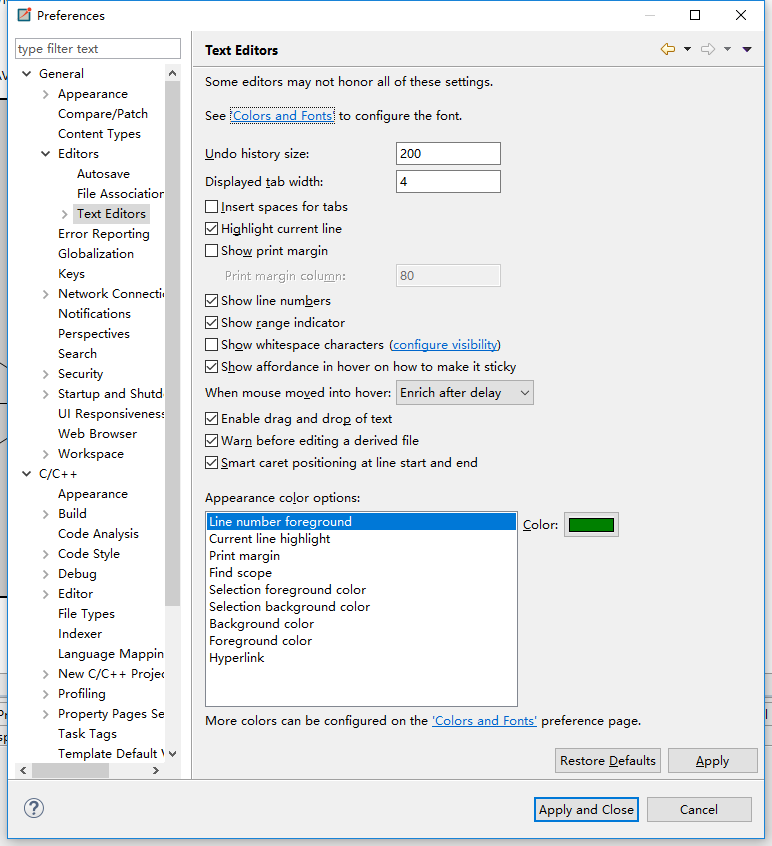
\includegraphics[keepaspectratio,width=\textwidth,height=0.75\textheight]{../img/chapter3/picture3-3-2.png}
\caption{其他设置界面}
\end{figure}

在这一界面中,我们Tab键宽度、显示行号或者当前行背景,其他设置读者可自行编辑看看。

\section{本章小结}
\label{本章小结}

\&\#160; \&\#160; \&\#160; \textbf{OMNeT++}仿真平台基于Eclipse,相关编译、工程设置与其他软件不同,且难找,本章列出仿真时读者可能需要用到的相关设置。

\chapter{OMNeT++仿真类}
\label{omnet仿真类}

在完成第五章后,考虑需要在之前加一章节关于OMNeT++类说明,在这个仿真软件中,主要使用的语言是C++,因此大多数数据类型是类或者结构,本章还是走其他技术书一样的老路线,注释这些数据类型,对类成员函数进行说明,可能与第五章有些重复的地方,但是其五章更多的偏向于实际应用,可能读者看过这里后,会发现OMNeT++接口是真好用。

\section{类说明}
\label{类说明}

\subsection{cModule}
\label{cmodule}

为了能更好的解释这个的库的使用,程序清单4.1为类cModule原型,cModule类在OMNeT++中表示一个节点的对象,这个节点可以是复合节点或者简单节点,通过这个类,程序员可以访问描述这个节点的.ned文件中设置的参数,或者是由omnetpp.ini传入的参数。简而言之,我们最后就是面向这些类进行网络设计。

\begin{lstlisting}[language=c]
程序清单4.1
class SIM_API cModule : public cComponent //implies noncopyable
{
    friend class cGate;
    friend class cSimulation;
    friend class cModuleType;
    friend class cChannelType;

  public:
    /* 门迭代器 */
    GateIterator

    /* 复合模块的子模块迭代器 */
    SubmoduleIterator

    /* 模块信道迭代器 */
    ChannelIterator

  public:
    virtual void callRefreshDisplay() override;

    virtual const char *getFullName() const override;

    virtual std::string getFullPath() const override;

    virtual bool isSimple() const;

    // 返回模块的父模块,对于系统模块,返回nullptr
    virtual cModule *getParentModule() const override;

    // 如何模块是使用向量的形式定义的,返回true
    bool isVector() const  {return vectorSize>=0;}

    // 返回模块在向量中的索引
    int getIndex() const  {return vectorIndex;}

    // 返回这个模块向量的大小,如何该模块不是使用向量的方式定义的,返回1
    int getVectorSize() const  {return vectorSize<0 ? 1 : vectorSize;}

    // 与getVectorSize()功能相似
    _OPPDEPRECATED int size() const  {return getVectorSize();}

    // 检测该模块是否有子模块
    virtual bool hasSubmodules() const {return firstSubmodule!=nullptr;}

    // 寻找子模块name,找到返回模块ID,否则返回-1
    // 如何模块采用向量形式定义,那么需要指明index
    virtual int findSubmodule(const char *name, int index=-1) const;

    // 直接得到子模块name的指针,没有这个子模块返回nullptr
    // 如何模块采用向量形式定义,那么需要指明index
    virtual cModule *getSubmodule(const char *name, int index=-1) const;

    /* 一个更强大的获取模块指针的接口,通过路径获取 */
    virtual cModule *getModuleByPath(const char *path) const;

    /*
     * 门的相关操作
     */

    // 检测是否有门
    virtual bool hasGate(const char *gatename, int index=-1) const;

    // 寻找门,如果没有返回-1,找到返回门ID
    virtual int findGate(const char *gatename, int index=-1) const;

    // 通过ID得到门地址,目前我还没有用到过
    const cGate *gate(int id) const {return const_cast<cModule *>(this)->gate(id);}

    // 删除一个门(很少用)
    virtual void deleteGate(const char *gatename);

    //返回模块门的名字,只是基本名字(不包括向量门的索引, "[]" or the "$i"/"$o")
    virtual std::vector<const char *> getGateNames() const;

    // 检测门(向量门)类型,可以标明"$i","$o"
    virtual cGate::Type gateType(const char *gatename) const;

    // 检测是否是向量门,可以标明"$i","$o"
    virtual bool isGateVector(const char *gatename) const;

    // 得到门的大小,可以指明"$i","$o"
    virtual int gateSize(const char *gatename) const;

    /*
     * 公用的
     */
    // 在父模块中寻找某个参数,没找到抛出cRuntimeError
    virtual cPar& getAncestorPar(const char *parname);

    // 设置是否在此模块的图形检查器上请求内置动画。
    virtual void setBuiltinAnimationsAllowed(bool enabled) {setFlag(FL_BUILTIN_ANIMATIONS, enabled);}

    // 删除自己
    virtual void deleteModule();

    // 移动该模块到另一个父模块下,一般用于移动场景。规则较复杂,可到原头文件查看使用说明
    virtual void changeParentTo(cModule *mod);
};
\end{lstlisting}

\textbf{cModule}是OMNeT++中用于代表一个模块的对象实体,如果你在编写网络仿真代码时,这个模块可以是简单模块或者复合模块,当需要得到这个模块相关属性时可以考虑到这个\textbf{cModule}类里边找找,说不定有意外的惊喜,也许有现成的函数实现你需要的功能。下面将这个类原型解剖看看:

\begin{itemize}
\item \textbf{迭代器:GateIterator}

\end{itemize}

\begin{lstlisting}[language=c]
usage:
for (cModule::GateIterator it(module); !it.end(); ++it) {
        cGate *gate = *it;
        ...
}
\end{lstlisting}

该迭代器可用于遍历模块\textbf{module}的门向量,得到该门可用于其他作用。

\begin{itemize}
\item \textbf{迭代器:SubmoduleIterator}

\end{itemize}

\begin{lstlisting}[language=c]
usage:
for (cModule::SubmoduleIterator it(module); !it.end(); ++it) {
        cModule *submodule = *it;
        ...
}
\end{lstlisting}

对于一个复合模块,包括多个简单模块或者复合模块,可使用该迭代器进行遍历操作,在第五章涉及到这个迭代器的使用。

\begin{itemize}
\item \textbf{迭代器:ChannelIterator}

\end{itemize}

\begin{lstlisting}[language=c]
usage:
for (cModule::ChannelIterator it(module); !it.end(); ++it) {
        cChannel *channel = *it;
        ...
}
\end{lstlisting}

可用于遍历该模块的所有的信道。

\subsection{cPar}
\label{cpar}

\textbf{cPar}同样是我们设置网络时不可避免的类,通过cPar得到节点在网络拓扑文件和配置文件中设置的参数,浏览完cPar所有成员函数,可以看出cPar基本提供了网络设计者想要的所有数据转换接口。

\begin{lstlisting}[language=c]
class SIM_API cPar : public cObject
{
    friend class cComponent;
  public:
    // 返回参数的名字
    virtual const char *getName() const override;

    // 以字符串的形式返回参数
    virtual std::string str() const override;

    virtual cObject *getOwner() const override; // note: cannot return cComponent* (covariant return type) due to declaration order

    Type getType() const;

    static const char *getTypeName(Type t);

    bool isNumeric() const;

    bool isVolatile() const;

    bool isExpression() const;

    bool isShared() const;

    bool isSet() const;

    cPar& setBoolValue(bool b);

    cPar& setLongValue(long l);

    cPar& setDoubleValue(double d);

    cPar& setStringValue(const char *s);

    cPar& setStringValue(const std::string& s)  {setStringValue(s.c_str()); return *this;}

    cPar& setXMLValue(cXMLElement *node);

    bool boolValue() const;

    long longValue() const;

    double doubleValue() const;

    const char *getUnit() const;

    const char *stringValue() const;

    std::string stdstringValue() const;

    cXMLElement *xmlValue() const;

    void parse(const char *text);

    // 与stdstringValue()功能一样
    operator std::string() const  {return stdstringValue();}

    // 与xmlVlaue()等同。注意:返回对象树的生命周期被限制了,具体看xmlValue说明。
    operator cXMLElement *() const  {return xmlValue();}
};
\end{lstlisting}

\subsection{cGate}
\label{cgate}

如果你需要在网络仿真运行时,动态实现两个节点之间的连接或者断开,那么你就需要在程序中用到这个类。

\begin{lstlisting}[language=c]
class SIM_API cGate : public cObject, noncopyable
{
    friend class cModule;
    friend class cModuleGates;
    friend class cPlaceholderModule;

  public:
    cGate *prevGate;    // previous and next gate in the path
    cGate *nextGate;

    static int lastConnectionId;

    static void clearFullnamePool();

    // internal
    void installChannel(cChannel *chan);

    // internal
    void checkChannels() const;

    /* 例如返回门out */
    virtual const char *getName() const override;

    /* 与getName()不同,需要返回门索引,例如out[4] */
    virtual const char *getFullName() const override;

    /**
     * This function is called internally by the send() functions and
     * channel classes' deliver() to deliver the message to its destination.
     * A false return value means that the message object should be deleted
     * by the caller. (This is used e.g. with parallel simulation, for
     * messages leaving the partition.)
     */
    virtual bool deliver(cMessage *msg, simtime_t at);

    cChannel *connectTo(cGate *gate, cChannel *channel=nullptr, bool leaveUninitialized=false);

    void disconnect();

    cChannel *reconnectWith(cChannel *channel, bool leaveUninitialized=false);

    const char *getBaseName() const;

    const char *getNameSuffix() const;

    cProperties *getProperties() const;

    Type getType() const  {return desc->getTypeOf(this);}

    static const char *getTypeName(Type t);

    cModule *getOwnerModule() const;

    int getId() const;

    bool isVector() const  {return desc->isVector();}

    int getIndex() const  {return desc->indexOf(this);}

    int getVectorSize() const  {return desc->gateSize();}

    cChannel *getChannel() const  {return channel;}

    cChannel *getTransmissionChannel() const;

    cChannel *findTransmissionChannel() const;

    cChannel *getIncomingTransmissionChannel() const;

    cChannel *findIncomingTransmissionChannel() const;
  
    cGate *getPreviousGate() const {return prevGate;}

    cGate *getNextGate() const   {return nextGate;}

    cDisplayString& getDisplayString();

    void setDisplayString(const char *dispstr);
};
\end{lstlisting}

\subsection{cTopology}
\label{ctopology}

\subsection{cExpression}
\label{cexpression}

\subsection{EV类}
\label{ev类}

一个对调试程序有帮助的类。

\begin{lstlisting}[language=c]
class SIM_API cLog
{
  public:
    static LogLevel logLevel;

    static const char *getLogLevelName(LogLevel logLevel);

    static LogLevel resolveLogLevel(const char *name);
};

#define EV_LOG(logLevel, category) OPP_LOGPROXY(getThisPtr(), logLevel, category).getStream()

#define EV        EV_INFO

#define EV_FATAL  EV_LOG(omnetpp::LOGLEVEL_FATAL, nullptr)

#define EV_ERROR  EV_LOG(omnetpp::LOGLEVEL_ERROR, nullptr)

#define EV_WARN   EV_LOG(omnetpp::LOGLEVEL_WARN, nullptr)

#define EV_INFO   EV_LOG(omnetpp::LOGLEVEL_INFO, nullptr)

#define EV_DETAIL EV_LOG(omnetpp::LOGLEVEL_DETAIL, nullptr)

#define EV_DEBUG  EV_LOG(omnetpp::LOGLEVEL_DEBUG, nullptr)

#define EV_TRACE  EV_LOG(omnetpp::LOGLEVEL_TRACE, nullptr)

#define EV_C(category)        EV_INFO_C(category)

#define EV_FATAL_C(category)  EV_LOG(omnetpp::LOGLEVEL_FATAL, category)

#define EV_ERROR_C(category)  EV_LOG(omnetpp::LOGLEVEL_ERROR, category)

#define EV_WARN_C(category)   EV_LOG(omnetpp::LOGLEVEL_WARN, category)

#define EV_INFO_C(category)   EV_LOG(omnetpp::LOGLEVEL_INFO, category)

#define EV_DETAIL_C(category) EV_LOG(omnetpp::LOGLEVEL_DETAIL, category)

#define EV_DEBUG_C(category)  EV_LOG(omnetpp::LOGLEVEL_DEBUG, category)

#define EV_TRACE_C(category)  EV_LOG(omnetpp::LOGLEVEL_TRACE, category)
}
\end{lstlisting}

\section{虚函数}
\label{虚函数}

\subsection{initialize函数}
\label{initialize函数}

\subsection{handleMessage函数}
\label{handlemessage函数}

\subsection{refreshDisplay函数}
\label{refreshdisplay函数}

\subsection{finish函数}
\label{finish函数}

\section{本章小结}
\label{本章小结}

本章对OMNeT++中提供的相关类进行了描述和说明,阅读相关头文件是掌握OMNeT++仿真有效方法。

\chapter{OMNeT++仿真技巧}
\label{omnet仿真技巧}

欢迎读者来到第五章的学习,本章打算从工程应用的角度,结合现有的仿真经验分享一些技巧,用套路二字来形容也不为过。
本章涉及的内容包括信道模型应用、节点分布相关、节点之间如何建立通信以及门向量的相关设置,同时也会涉及以上代码相关的说明,简而言之,本章采用情景分析的方法进行说明。也许你会发现本章好多内容可以在OMNeT++社区提供的Simulation Manual手册中发现,所以推荐读者后续再阅读Simulation Manual手册进行深度研究。

\section{设计技巧}
\label{设计技巧}

\subsection{技巧一:信道模型很重要}
\label{技巧一:信道模型很重要}

 据说理想的运放可以摧毁整个地球,那么是不是理想的充电宝是不是充不满电,偏题了,那么理想的信道呢?当初初次使用OMNeT++时,遇到一个问题:

\begin{itemize}
\item >在节点之间传输消息的时候,如何加快消息的传输速度?当节点数量较大的时候,需要较快的实现消息传送的效果。

\end{itemize}

有此疑问是在运行社区提供的相关工程时发现在他们的的仿真场景中,两个节点似乎可以同时发送消息出去,给人一种并行运行的感觉,让我不得不怀疑是不是需要调用并行接口才能达到这种效果,并且也发现他们的仿真程序运行时间特别小,换句话说就是接近现实的时间级,而我的仿真程序中两个节点传输一个消息都到秒级了,问题很大。
最后发现这个问题与信道模型有关,也与下一小节的send函数相关。在OMNeT++中仿真的时候,如果没有添加信道模型,消息在两个节点之间传输线就是理想的信道模型,这个仿真信道会影响什么呢?

\begin{itemize}
\item 仿真结果

\item 仿真现象

\end{itemize}

影响仿真结果好理解,仿真现象呢,那我们来看看仿真模型:

\begin{lstlisting}[language=c]
channel Channel extends DatarateChannel
{
    delay = default(uniform(20ns, 100ns));
    datarate = default(1000Mbps);
}
\end{lstlisting}

以上代码是一个简单的信道模型,将这个信道加入到传输线上将会有意想不到的效果。

\subsection{技巧二:send函数有套路}
\label{技巧二:send函数有套路}

不知道读者有时候有没有感觉到send函数很麻烦,send函数用于两个模块之间的消息传输,但是当我们需要发送多条消息的时候,我们不能使用for循环直接就上,其主要原因就上我们使用send函数发送的消息还没有到达目的节点,此时我们不能使用send函数发送下一条消息,那么怎么办呢?这里有两种方案:

\begin{itemize}
\item 利用scheduleAt函数

\end{itemize}

\begin{lstlisting}[language=c]
void Node::handleMessage(cMessage* msg)
{
    if(msg->isSelfMessage()){
        if(msg->getKind()==SMSG_INIT){
                ...
                ...
            cMessage* cloudMsg = new cMessage("hello");
            cloudMsg->setKind(SMSG_INIT);//设置节点类型
            scheduleAt(simTime()+0.01,cloudMsg); //调度一个事件,发送消息给自己
        }
    }
}
\end{lstlisting}

通过使用scheduleAt函数使仿真时间走动,完成上一个消息的完成,这里补充一点,如果读者想使用延时来等待消息传输完成是不可行的,因为使用这种方法仿真时间是不会走动的。例如下面一段代码:

\begin{lstlisting}[language=c]
time1 = simTime();
func();
time2 = simTime();
\end{lstlisting}

在上面这段代码中我们的使用func函数想使时间走动,但是实验结果告诉我们:
\$time1==time2\$,
经过多次多个地方验证,发现在OMNeT++中如果不调用与仿真时间相关的函数,仿真时间是不会走动的,与上面的实验现象是一致的。因此为了实现仿真时间的走动我们可以采用上面scheduleAt函数自我调度一个时间然后再发送下一个消息。

\begin{itemize}
\item 一定要采用send函数呢?

\end{itemize}

上述采用scheduleAt的方法太麻烦,需要\textbf{new}一个消息,然后还需要定义一个SMSG\_INIT,另外无端增多handleMessage函数内容,这种方法的确不是特别简洁。这里再分享另一种方法:

\begin{lstlisting}[language=c]
cPacket *pkt = ...; // packet to be transmitted
cChannel *txChannel = gate("out")->getTransmissionChannel();
simtime_t txFinishTime = txChannel->getTransmissionFinishTime();
if (txFinishTime <= simTime())
{
    // channel free; send out packet immediately
    send(pkt, "out");
}
else
{
    // store packet and schedule timer; when the timer expires,
    // the packet should be removed from the queue and sent out
    txQueue.insert(pkt);
    scheduleAt(txFinishTime, endTxMsg);
}

\end{lstlisting}

上面的代码用于通过out门发送一个pkt包,但是在传输前需要得到该门上传输的消息的完成时间,需要注意的是当txFinishTime为-1时,说明该门没有消息传输,可以直接发送,如果txFinishTime为一个大于0的值,说明有消息正在传输,需要等待。所以在判断时我们采用\$txFinishTime <= simTime()\$。
通过这种方式,我们可以在for循环中发送多个消息。但是对于有些需求不得不使用scheduleAt函数完成。

\begin{itemize}
\item 提一提sendDirect函数!

\end{itemize}

\begin{lstlisting}[language=c,caption=My]
sendDirect(cMessage *msg, cModule *mod, int gateId)
sendDirect(cMessage *msg, cModule *mod, const char *gateName, int index=-1)
sendDirect(cMessage *msg, cGate *gate)

sendDirect(cMessage *msg, simtime_t propagationDelay, simtime_t duration,
           cModule *mod, int gateId)
sendDirect(cMessage *msg, simtime_t propagationDelay, simtime_t duration,
           cModule *mod, const char *gateName, int index=-1)
sendDirect(cMessage *msg, simtime_t propagationDelay, simtime_t duration,
           cGate *gate)

\end{lstlisting}

对于其他send类似的函数都是有线的传输方式,需要我们将节点连接才能发送消息,那么如何实现无线的发送方式呢?这个也正是OMNeT++中wireless仿真程序中使用的函数,该函数的参数与其他send函数不同,它需要指定目的节点,以及目的节点的门。相关详细可以阅读INET库代码。
这里有一个问题,当采用前三个函数进行消息传输时,传输的效果为一个圆点,如图\textbf{5--1}所示:

\begin{figure}[htbp]
\centering
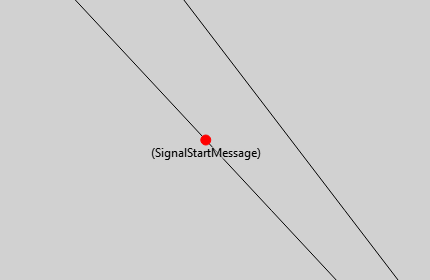
\includegraphics[keepaspectratio,width=\textwidth,height=0.75\textheight]{../img/chapter5/图-红点.png}
\caption{普通传输效果图}
\end{figure}

如果在设计网络时,需要将包传输效果设置成图5--2所示,对于有线连接和无线连接的两个节点方法不同,对于有线连接的send函数无法在函数的参数上设置。需要在网络拓扑连接时设置好信道,如代码段5--1所示:

\begin{lstlisting}[language=c]
channel Channel extends DatarateChannel
{
    delay = default(uniform(20ns, 100ns));
    datarate = default(2000Mbps);
}

\end{lstlisting}

对于无线连接的sendDirect函数,要想达到相同的效果,就没有设置channel一说了,在使用sendDirect函数时,有三个重载函数包括有两个参数simtime\_t propagationDelay\slash simtime\_t duration,一个是传播延时时间和持续时间,通过设置这两个参数可以达到图5--2的效果。

\begin{figure}[htbp]
\centering
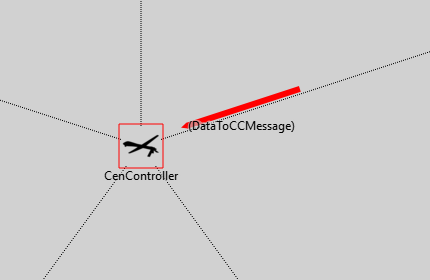
\includegraphics[keepaspectratio,width=\textwidth,height=0.75\textheight]{../img/chapter5/图-帧长图.png}
\caption{设置传输延迟和持续时间}
\end{figure}

\subsection{技巧三:如何访问同一级的其他模块}
\label{技巧三:如何访问同一级的其他模块}

在设计网络拓扑时,我们有时需要在一个模块中直接访问同一级其他模块的相关参数,不再经过消息之间传输进行传输。这种接口在OMNeT++下也被提供了,如下一个代码示例:

\begin{lstlisting}[language=c]
cModule *parent = getParentModule();

// 取出父模块下的beBuffer模块
cModule *psubmodBE = parent->getSubmodule("beBuffer");
BEBuffer *pBEBuffer = check_and_cast<BEBuffer *>(psubmodBE);

cModule *psubmodRC = NULL;
RCBuffer *pRCBuffer = NULL;
// 取出父模块下的rcBuffer模块
psubmodRC = parent->getSubmodule("rcBuffer");
pRCBuffer = check_and_cast<RCBuffer *>(psubmodRC);

\end{lstlisting}

上面的代码片段主要通过getParentModule和getSubmodule两个接口得到指向目的模块的指针,得到指针相当于我们拿到了这个目的模块的所有,需要注意的是这种方式的前提是目的模块是一个简单模块,需要与复合模块区分开,在OMNeT++中复合模块只有对应的\textbf{.ned}文件,其描述方式如下:

\begin{lstlisting}[language=c]
module Node{
        parameters:
    	...
	gates:
	...
}
\end{lstlisting}

而简单模块有三个文件:\textbf{.nde、.cc、.h},其.ned文件中描述方式如下:

\begin{verbatim}

simple Node{
	parameters:
    	...
	gates:
	...
}
\end{verbatim}

因此对于没有.cc\slash .h文件的复合模块,在编写代码时就没有对应的C++类,因此使用上述方法就出现问题,无法事先知道指针类型,那么对于复合模块的访问,我们可以通过下面的代码实现:

\begin{lstlisting}[language=c]
// 得到当前父模块下的所以模块
for(cModule::SubmoduleIterator iter(getParentModule()); !iter.end(); iter++){
        string ES = string("ES");
        cModule *submodule = *iter;
        string ESnode = string(submodule->getFullName(),0,2);
        // 判断是否是ES节点
        if(ESnode == ES){
                // 访问父模块参数
                string realname = string(submodule->getFullName());
                EScpu += submodule->par("cpu").longValue();
                ESmem += submodule->par("mem").longValue();

                cout<<EScpu<<" "<<ESmem<<endl;
        }
        else{
                continue;
        }
}
\end{lstlisting}

上面的代码段涉及到了OMNeT++下的SubmoduleIterator迭代器,该迭代器在较多的库中都有使用,比如:INET,当然这种方式可以经过简单的修改也可以对简单的模块进行访问。在上面的代码段中,getParentModule()指明是当前模块的父模块,该代码目的就是在当前简单模块中,得到同一父模块下的ES复合模块的cpu\slash mem两个参数。

\subsection{技巧四:遍历所有模块}
\label{技巧四:遍历所有模块}

在有些场景下,我们需要遍历所有节点,甚至是复合节点内部的模块,代码示例如下:

\begin{lstlisting}[language=c]
/*
 * 在所有节点中寻找一个ID 等于当前模块的headId号的模块
 */
void Node::doNext()
{
    cModule *parent = getParentModule();
    cModule *mod,*Head,*midmod;

    //网络中的所有节点都遍历一次,包括复合模块下的子模块
    for(int i=1;i<=cSimulation::getActiveSimulation()->getLastComponentId();i++){
        int number_of_Bees = cSimulation::getActiveSimulation()->getLastComponentId();
        cSimulation *simobj = cSimulation::getActiveSimulation();
        //这里需要优化
        mod = cSimulation::getActiveSimulation()->getModule(i);
        if(strcmp(mod->getName(),"CenController") == 0){
            //如果遍历到一个模块名为CenController的节点
            continue;
        }
        else{
            int j=0;
            while(1){
                string modname = cSimulation::getActiveSimulation()->getModule(i)->getName();
                midmod=cSimulation::getActiveSimulation()->getModule(i);
                Head=midmod->getSubmodule(this->clustername.c_str(),j)->getSubmodule("Wireless");
                if(((Node*)Head)->myId == this->headId){
                    //找到簇头节点,退出while循环
                    break;
                }
                j++;
            }
            // 在到满足条件的Head节点,开始执行相关操作
            ...
            ...
            ...
            break;
        }
    }
}

\end{lstlisting}

在上面的代码段中,可能有些诸如“Wireless”相关的过程与我实验源代码本身功能相关,本例只提供一种可参考的代码,具体运用于读者自己的项目中还需要做部分修改。为了让读者更快的掌握这种方法,下面就代码段中的重要接口做一个简单的分析:

\begin{itemize}
\item \textbf{for(int i=1;i<=cSimulation::getActiveSimulation()->getLastComponentId();i++)}

\end{itemize}

这一句for循环遍历当前网络场景中的模块,只遍历仿真场景中的节点,不包括节点内部的模块,下面结合一个网络拓扑文件说明:

\begin{lstlisting}[language=c]
network simplenet
{
    parameters:
        ...
        ...
    submodules:

        node1[x]: typeA {
            parameters:
                ...
        }

        node2[y]: typeB{
            parameters:
                ...
        }

        node3[z]: typeD {
            parameters:
                ...
        }

    connections allowunconnected:
        ...
        ...
}

\end{lstlisting}

对于上述网络拓扑,使用上面的for循环只能遍历node1\slash node2\slash node3,对于它们内部的子模块不在其内。当最终需要寻找的模块是其中一个的子模块,需要先遍历父模块,然后使用getSubmodule函数遍历子模块。

\begin{itemize}
\item midmod = cSimulation::getActiveSimulation()->getModule(i)

\end{itemize}

紧接着上面的for循环,得到第\textbf{i}个模块的地址,如果该模块在网络中描述是用向量的方式需要使用:
$$getSubmodule(“node_name”,j)$$
即可得到node\_name{[j]}所代表的模块。

\begin{itemize}
\item getSubmodule(``modname'')

\end{itemize}

该接口似乎使用频率较高,如何得到一个复合模块的指针,即可通过该接口得到内部子模块的指针,然后访问相关数据。

\subsection{技巧五:如何得到某一个模块引用的ned路径}
\label{技巧五:如何得到某一个模块引用的ned路径}

为什么需要在一个程序中得到该``.ned''引用的路径呢?因为在OMNeT++中,我们在设计一个复合模块的内部结构时,可以直接采用图形的方式编辑,相当于我们可以直接拖动设计好的简单模块到复合模块中,而有些简单模块在不同的复合模块中其功能还有所不同,因此在为该简单模块编写.cc文件时,我们需要检测一下当前本模块在什么模块下使用的,比如是在端系统还是交换机。得到一个模块的引用路径,其实就是一个接口函数的事,如下代码段:

\begin{lstlisting}[language=c]
cModule *parent = getParentModule();
const char *name = parent->getNedTypeName();

if (strcmp(name, "SimpleNetwork.Node.SimpleNode") == 0){
    cGate *outgate = gate("line$o");
    cChannel *chan = outgate->findTransmissionChannel();
    linkspeed = chan->getNominalDatarate();

}
else if (strcmp(name, "SimpleNetwork.Switch.SwitchPort") == 0){
    //int id = parent->findGate("line$o");
    cGate *outgate = parent->gate("line$o");
    cChannel *chan = outgate->findTransmissionChannel();
    linkspeed = chan->getNominalDatarate();
}

\end{lstlisting}

该接口函数便是getNedTypeName,得到完整的路径后,使用c库函数strcmp进行判断即可。

\subsection{技巧六:使用cTopology类遍历拓扑初始化路由表}
\label{技巧六:使用ctopology类遍历拓扑初始化路由表}

这是个好东西,其实在OMNeT++中其实提供的大量的接口函数,只是在不知道的前提下写相似的功能函数比较麻烦,这个接口函数完美解决我们寻找路由的门问题,在使用send函数传输消息的时候只要知道我们传输的目的节点便可,直接利用一个路由表即可,代码示例如下:

\begin{lstlisting}[language=c]
/*
 * 探测交换机网络的拓扑
 */
void Router::TopoFind()
{
    cTopology *topo = new cTopology("topo");

    topo->extractByNedTypeName(cStringTokenizer("SimpleNetwork.Node.SimpleNode SimpleNetwork.Switch.SimpleSwitch").asVector());

    EV << "cTopology found " << topo->getNumNodes() << " nodes\n";

    //得到表示本节点的对象
    cTopology::Node *thisNode = topo->getNodeFor(getParentModule());

    // find and store next hops
    for (int i = 0; i < topo->getNumNodes(); i++){
        if (topo->getNode(i) == thisNode)
            continue; // skip ourselves
        //采用迪杰斯特拉算法计算到节点i的最短距离
        topo->calculateUnweightedSingleShortestPathsTo(topo->getNode(i));
        //本节点与外界连接的通道
        if (thisNode->getNumPaths() == 0)
            continue; // not connected

        cGate *parentModuleGate = thisNode->getPath(0)->getLocalGate();
        int gateIndex = parentModuleGate->getIndex();
        int address = topo->getNode(i)->getModule()->par("address");
        rtable[address] = gateIndex;
        EV << "  towards address " << address << " gateIndex is " << gateIndex  << endl;
    }
    delete topo;
}

\end{lstlisting}

该函数有三个比较重要的步骤:

\begin{itemize}
\item {[1]} \textbf{extractByNedTypeName}

\end{itemize}

为了得到一个路由表,我们需要指明需要遍历的节点类型。该函数便是指明遍历哪些节点。

\begin{itemize}
\item {[2]} \textbf{calculateUnweightedSingleShortestPathsTo}

\end{itemize}

得到路由表也涉及到路由算法的选择,在\textbf{ctopology.h}文件中有以下两个路由算法可供选择:

\begin{lstlisting}[language=c]
/** @name Algorithms to find shortest paths. */
/*
* To be implemented:
*    -  void unweightedMultiShortestPathsTo(Node *target);
*    -  void weightedMultiShortestPathsTo(Node *target);
*/

//@{

/**
* Apply the Dijkstra algorithm to find all shortest paths to the given
* graph node. The paths found can be extracted via Node's methods.
*/
virtual void calculateUnweightedSingleShortestPathsTo(Node *target);

/**
* Apply the Dijkstra algorithm to find all shortest paths to the given
* graph node. The paths found can be extracted via Node's methods.
* Uses weights in nodes and links.
*/
virtual void calculateWeightedSingleShortestPathsTo(Node *target);

\end{lstlisting}

代入参数就是目的节点地址,其他内容读者可自行探索。

\begin{itemize}
\item {[3]} \textbf{topo->getNode(i)->getModule()->par(``address'');}

\end{itemize}

这里比较重要的便是“address”形参,在以太网中相当于\textbf{IP}地址,最终得到的rtable{[]}表其索引就是目的地址的address,索引对应的值就是该节点的门,从该门出去到目的节点路径最短。

\subsection{技巧七:如何使用OpenSceneGraph}
\label{技巧七:如何使用openscenegraph}

其实在OMNeT++中是可以直接使用OpenSceneGraph的,可怜的我尝试了安装了一下午,才知道OMNet++已经支持OpenSceneGraph了,以后补充这一点可以看:

\begin{quote}
omnetpp-5.2\slash doc\slash manual\slash index.html\#sec:graphics:opp-api-for-osg 
\end{quote}

samples里已经有支持三维显示的仿真程序了,读者可自行运行看。

\subsection{技巧八:如何多次利用同一个msg}
\label{技巧八:如何多次利用同一个bmsgb}

在OMNeT++中,凡是使用scheduleAt调度的消息属于Self-Messages,其作用是用在模块本身调度事件使用的。有时需要利用同一个msg,但是中间必须使用cancelEvent函数取消掉上次,如下片段:

\begin{lstlisting}[language=c]
//cMessage *msg
if (msg->isScheduled())
    cancelEvent(msg);
scheduleAt(simTime() + delay, msg);
\end{lstlisting}

该代码段没有什么特别大的功能,主要是重复利用已经定义好的msg变量。

\subsection{技巧九:initialize函数的不同}
\label{技巧九:initialize函数的不同}

在每一个简单模块对应的.cc\slash .h文件中会有一个initialize函数,其功能是在仿真程序开始执行前将会执行的函数,与类的构造函数不同,引出的问题就是:

\begin{quote}
如果在其他成员函数中给一个指针数组成员赋值,当离开这个函数后,该指针数组值将会回到原来的值,该函数赋的值没有任何作用,但是如果在initialize函数中初始化这个指针数组,将会达到我们想要的结果。
\end{quote}

\subsection{技巧十:如何从仿真场景读取节点坐标}
\label{技巧十:如何从仿真场景读取节点坐标}

也许作者的用词不明,这里的仿真场景指的是运行仿真后出现的仿真界面。必须提到的是这个OMNeT++的仿真场景,节点在该场景上的位置,不一定是它的属性里边的地址,它们可以不同,感觉似乎是OMNeT++开发者提供的缺口,不知这个是好还是坏,但是好消息就是这些开发者提供了读取场景上节点属性的坐标和在程序中设置该坐标(目的就是让这个显示坐标更新),简而言之,你的节点坐标更新需要你自己在程序中完成,OMNeT++不会自动帮你完成。程序5.2.9--1是关于读取坐标和更新场景坐标的显示的代码段:

\begin{lstlisting}[language=c]
程序5.2.9-1
// 按照最开始的网络拓扑(按圆形分布),得到每一个节点的坐标
auto parentdispStr = parents->getDisplayString();
this->xpos = atof(parentdispStr.getTagArg("p", 0));
this->ypos = atof(parentdispStr.getTagArg("p", 1));

coord_X.setDoubleValue(this->xpos); //将仿真界面上的xpos改变
coord_Y.setDoubleValue(this->ypos); //将仿真界面上的ypos改变
\end{lstlisting}

需要再次提示的是这个坐标读取的是显示的节点的坐标,与节点在仿真场景上显示的位置可能没有关系。

对于一个复合模块中的一个简单节点想获符合节点中的坐标以及该节点的移动速度时,可以利用inet中自带的iMobility模块即可以实现完成。具体的实现程序如下所示:

\begin{lstlisting}[language=c]
程序5.2.9-1
// 按照最开始的网络拓扑(按圆形分布),得到每一个节点的坐标
cModule *temp_NodeModule=this->getParentModule();
inet::IMobility *node_Mobility=check_and_cast<IMobility *>(temp_NodeModule->getSubmodule("mobility"));
Coord coord_Node=node_Mobility->getCurrentPosition();//获取节点的位置
double NodeX=coord_Node.x;
double NodeY=coord_Node.y;
Coord speed_Node=node_Mobility->getCurrentVelocity();//获取节点的速度
double  NodeVv=speed_Node.x;
double NodeVy=speed_Node.y;
\end{lstlisting}

\subsection{技巧十一:如何调用INET中的类}
\label{技巧十一:如何调用inet中的类}

有时候在仿真程序中有种需求:

\begin{quote}
需要在一个仿真程序中调用其他库中的函数,例如需要使用INET中相关类,那这时候的逻辑是什么?
\end{quote}

与在某一个工程下需要import INET中的NED模型,我们需要在工程的属性中Project References中勾上我们需要import的库,然后在工程的ned文件中添加ned模型路径。同时当我们设置了工程Project References,当编译该工程时,将会链接Project References中勾上的工程编译生成的库文件,其中涉及以下编译设置:

\begin{lstlisting}[language=c]
// macros needed for building Windows DLLs
#if defined(_WIN32)
#  define OPP_DLLEXPORT  __declspec(dllexport)
#  define OPP_DLLIMPORT  __declspec(dllimport)
#else
#  define OPP_DLLIMPORT
#  define OPP_DLLEXPORT
#endif

\end{lstlisting}

以上摘取自INET开源库中\textbf{platdefs.h\textbf{文件,其中比较重要的是当编译INET库时,编译默认选项会使用}\_\_declspec(dllexport)\textbf{,当另一个仿真工程(使用了}INET}库中的类)编译时,将会以**\_\_declspec(dllimport)\textbf{,因此工程不需要设置其他编译选项,但是需要将诸如}INET\textbf{编译生成的}dll\textbf{或者}a**拷贝一份到该工程目录下。

\begin{itemize}
\item 注意:

\end{itemize}

如果以上关系皆满足,再出现在链接工程的错误可能其其他导致的。

\section{可视化接口}
\label{可视化接口}

\subsection{设置消息传输颜色}
\label{设置消息传输颜色}

\subsection{设置节点}
\label{设置节点}

在设置节点前,先阅读以下代码:

\begin{lstlisting}[language=c,caption=an]
this->getDisplayString().setTagArg("i",1,"red");
\end{lstlisting}

由以上代码函数名基本可以猜想到该行代码可能是设置显示相关标记,但具体设置哪一种标记可能需要知道\textbf{setTagArg()\textbf{函数的参数意义。其中}i}代表所设置\textbf{Tags}类型,在**OMNeT++\textbf{中}Tags**类型包括:

\begin{itemize}
\item p -- positioning and layout

\item p -- positioning and layout

\item b -- shape (box, oval, etc.)

\item i -- icon

\item is -- icon size

\item i2 -- auxiliary or status icon

\item r -- range indicator

\item q -- queue information text

\item t -- text

\item tt -- tooltip

\end{itemize}

所以,根据以上列表得知prog-5.x将设置图标相关属性,接下来我们需要知道紧接着的两个参数含义:

\begin{lstlisting}[language=c]
@display("i=block/source,red,20")
\end{lstlisting}

从\textbf{ned}文件中节点显示设置可以看出,属性\textbf{i}后第1个参数为\textbf{red}(从0开始数),那么prog-5.x便是将\textbf{i}后第\textbf{i}个参数设置为\textbf{red},到这里我们对**setTagArg()**函数的使用便掌握了。

\section{调试技巧}
\label{调试技巧}

\subsection{gdb调试}
\label{gdb调试}

OMNeT++支持gdb调试,与其他IDE调试方式相似,不同之处在于,若在网络仿真原型中设有统计参数,需在配置文件\textbf{omnetpp.ini}中设置:

\begin{lstlisting}[language=c]

check-signals = false

\end{lstlisting}

若仿真过程中,未关闭\textbf{check-signals},调试过程将会发生统计参数内存分配问题。

\subsection{log日志类}
\label{log日志类}

由于OMNeT++所提供\textbf{EV}显示信息在关闭仿真程序后,无法查看,可采用日志类将仿真信息打印到文本文件(亦可将\textbf{cout}重定向到文件)。在这里分享一个作者在调试OMNeT++仿真程序时编写的日志类\textbf{logging}。
使用方法如下:

\begin{lstlisting}[language=c]
/* 声明 */
using namespace logging

logger variablename("path to file","filename"); 

/* 使用 */
logger<<"current simulation time = "<<simTime()<<endl;
\end{lstlisting}

下载地址:\href{https://github.com/wangrongwei/lazytools}{logging-class}\footnote{\href{https://github.com/wangrongwei/lazytools}{https:\slash \slash github.com\slash wangrongwei\slash lazytools}}

\subsection{技巧十二:如何实现跨模块进行调用函数或参数}
\label{技巧十二:如何实现跨模块进行调用函数或参数}

在进行仿真的过程中,难免用到跨模块的函数调用或者参数调用,本部分主要对这部分进行简单的介绍:
其大致思路如下:
1)从复合模块中的一个简单模块退到该简单模块的上一层,也就是其父模块;

\begin{lstlisting}[language=c]
cModule *temp_Module=this->getParentModule();
\end{lstlisting}

2) 从父模块中找到你所要找到包含你需要的函数的子模块,也就是简单模块;

\begin{lstlisting}[language=c]
App *temp_mobility=check_and_cast<App *>(temp_Module->getSubmodule("app"));
/* App表示子模块的类名称 ,app表示你所需要的模块*/
\end{lstlisting}

3)找到你所需要的模块之后,然后就可以获得你所需要的函数或参数变量;

\begin{lstlisting}[language=c]
if(this->mClusterHead==app->myAddress){
    if(!app->mIsClusterHead){//这就是获得其他模块中的参数
        app->mIsClusterHead=true;
    }
}
\end{lstlisting}

\subsection{技巧十三:如何实现节点消息的同时显示}
\label{技巧十三:如何实现节点消息的同时显示}

当一个节点对多个节点进行发送消息时,为了在视觉上看到消息同时从一个端口发出,只需要利用一个函数就可以解决:

\begin{lstlisting}[language=c]
simtime_t txFinishTime = gate("line$o")->getTransmissionChannel()->getTransmissionFinishTime();
if((txFinishTime == -1) || (txFinishTime < simTime())){
    //通过修改延迟可以使节点能够同时发送消息
    sendDirect(pk,0.001,0,allUAV[(int)pk->getDestAddr()],"port$i",address);
}
else{
        sendDirect(pk,txFinishTime-simTime(),0.5,allUAV[(int)pk->getDestAddr()],"port$i",address);
    }
\end{lstlisting}

需要注意:
1)该函数一定放在与外界相连接的简单模块,不然时看不到的;

最终的显示效果入下图所示
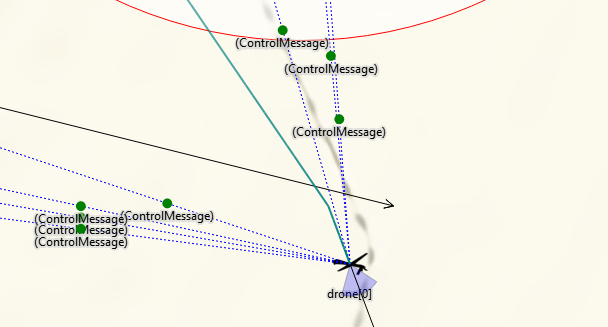
\includegraphics[keepaspectratio,width=\textwidth,height=0.75\textheight]{./../img/chapter5/5-1.png}

\section{本章小结}
\label{本章小结}

\textbf{OMNeT++\textbf{仿真内核提供的丰富的仿真接口,使用}OMNeT++\textbf{进行仿真,在掌握一定的}C++}编程方法以后,阅读 \&\#160; \textbf{OMNeT++}相关类的描述可能有意外的收获,找到合适的接口进行仿真。

\chapter{数据统计与仿真分析}
\label{数据统计与仿真分析}

OMNeT++有诸多工具对网络代码中统计的标量和矢量进行数据分析。
本章以一个AFDX网络的RC和BE消息的仿真结果为前提,依赖OMNeT++自带的工具集对这些结果进行分析,重点主要放在如何设置需要统计的标量和矢量?如何对最后的仿真结果进行操作得到我们想要的散点图、直方图等其他便于分析的数据图形。

\section{仿真结果有哪些}
\label{仿真结果有哪些}

先备注一下,每次运行完仿真后,将会产生三个文件:
.sca .vci .vec,点击.vec文件将会生成.anf文件,这个.anf文件当我们下一次重新运行仿真程序的时候,会更新,不需要删除后执行仿真程序。

\section{仿真结果的获取}
\label{仿真结果的获取}

在平常各种各样的仿真实验中,首先我们需要去获取所需的结果信息。在OMNeT++中有以下几种常用的获取仿真结果的方式,这里同时简单描述一下它们的用法。

\begin{itemize}
\item cLongHistogram:记录数据然后实现等距直方图 
定义:cLongHistogram hopCountStats;
我们可以对名称进行设置,如hopCountStats.setName(“hopcountStats”);
设置上限值:hopCountStats.setRangeAutoUpper(“0,10,1.5”);
记录数据:hopCountStats.collect(hopcount);
一些其他的属性如getMin()、getMax()、getMean()以及getStddev(),不做赘述。

\item cOutVector:获取输出向量
定义:cOutVector hopCountVector;
同样可以人为地对名称进行设置,比如hopCountVector.setName(“Hopcount”);
记录数据:hopCountVector.record(hopcount);
其中,record表示记录数据。缺少这一语句的话,不会有任何的数据输出。

\item recordScalar
输出程序中某个标量的值,直接调用即可。即
recordScalar(“string 输出名称”, 输出变量名);
仿真之后的result文件中会有以“string 输出名称”命名的文件。“输出变量名”为我们要输出查看的变量。recordScalar较为简单,一般在Finish()函数中使用。

\end{itemize}

\section{仿真结果分析}
\label{仿真结果分析}

每次仿真的结果都会存储在project下面的result文件夹中。
cOutVector: \textbackslash{}result\textbackslash{}xxx.vec
cLongHistogram: \textbackslash{}result\textbackslash{}xxx.sca

\begin{figure}[htbp]
\centering
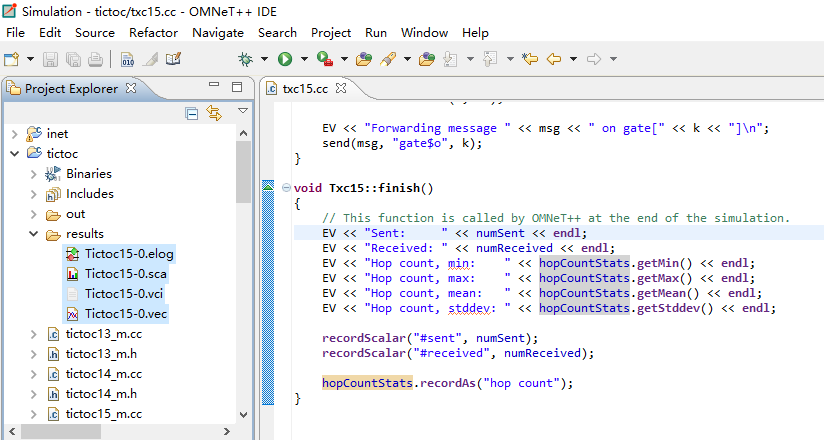
\includegraphics[keepaspectratio,width=\textwidth,height=0.75\textheight]{../img/chapter6/6-1.png}
\caption{doc目录}
\end{figure}

如图所示,Project Explorer中选中的文件就是我们的仿真结果。之后双击打开就可以查看里面的内容,这里我选择打开了vec文件。

\begin{figure}[htbp]
\centering
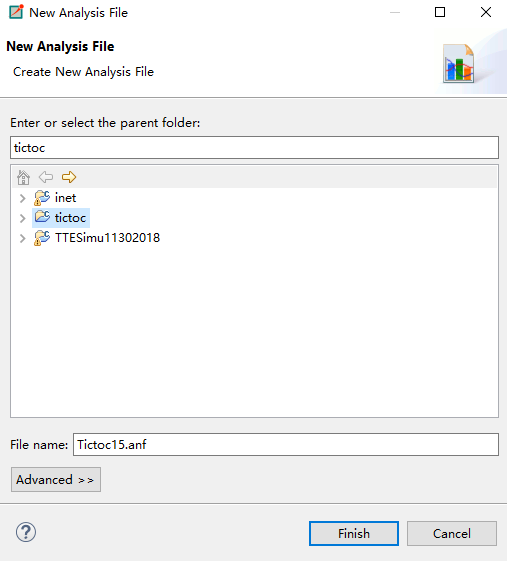
\includegraphics[keepaspectratio,width=\textwidth,height=0.75\textheight]{../img/chapter6/6-2.png}
\caption{doc目录}
\end{figure}

然后会让我们建立新的分析文件。点击finish即可

\begin{figure}[htbp]
\centering
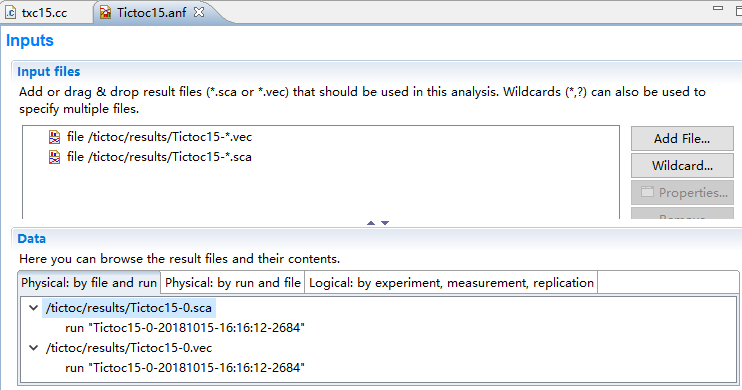
\includegraphics[keepaspectratio,width=\textwidth,height=0.75\textheight]{../img/chapter6/6-3.png}
\caption{doc目录}
\end{figure}

点击打开Data栏中vec下属的记录。Tictoc15网络中有6个节点,可以看到仿真对它们全部进行了记录

\begin{figure}[htbp]
\centering
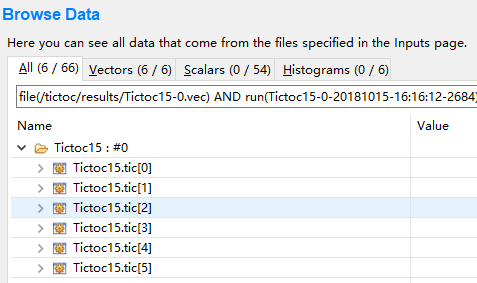
\includegraphics[keepaspectratio,width=\textwidth,height=0.75\textheight]{../img/chapter6/6-4.png}
\caption{doc目录}
\end{figure}

\begin{figure}[htbp]
\centering
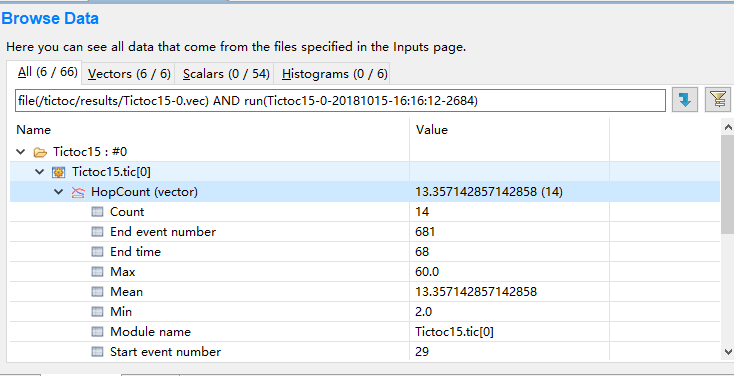
\includegraphics[keepaspectratio,width=\textwidth,height=0.75\textheight]{../img/chapter6/6-5.png}
\caption{doc目录}
\end{figure}

其实,观察选项卡就可以发现,这里我们就可以查看所有的结果了。由于笔者打开的是vec文件,所以只有输出向量。

\begin{figure}[htbp]
\centering
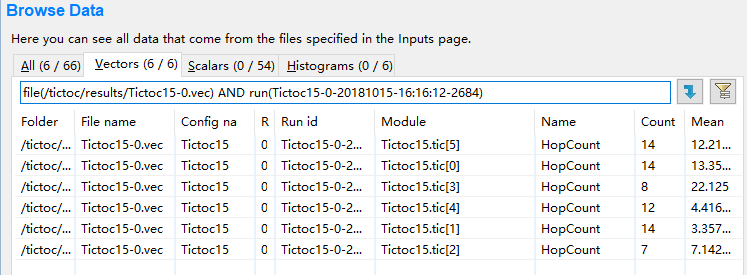
\includegraphics[keepaspectratio,width=\textwidth,height=0.75\textheight]{../img/chapter6/6-6.png}
\caption{doc目录}
\end{figure}

双击打开想查看的一行,如下所示:

\begin{figure}[htbp]
\centering
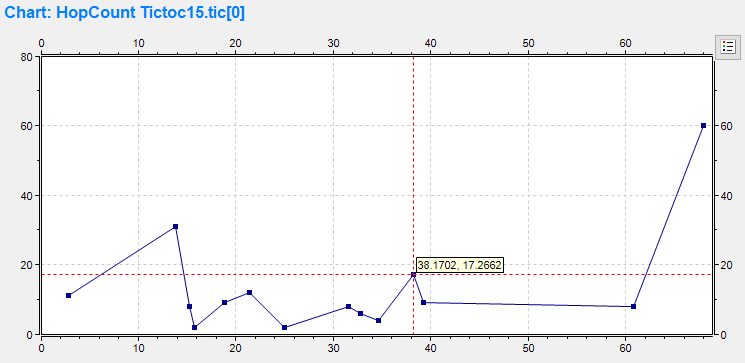
\includegraphics[keepaspectratio,width=\textwidth,height=0.75\textheight]{../img/chapter6/6-7.png}
\caption{doc目录}
\end{figure}

接下来我们打开sca文件查看直方图:

\begin{figure}[htbp]
\centering
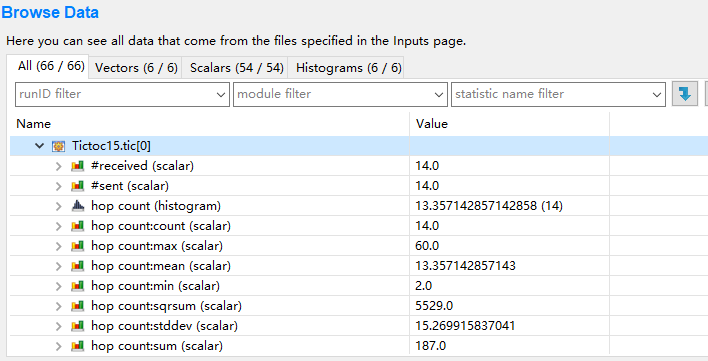
\includegraphics[keepaspectratio,width=\textwidth,height=0.75\textheight]{../img/chapter6/6-8.png}
\caption{doc目录}
\end{figure}

\begin{figure}[htbp]
\centering
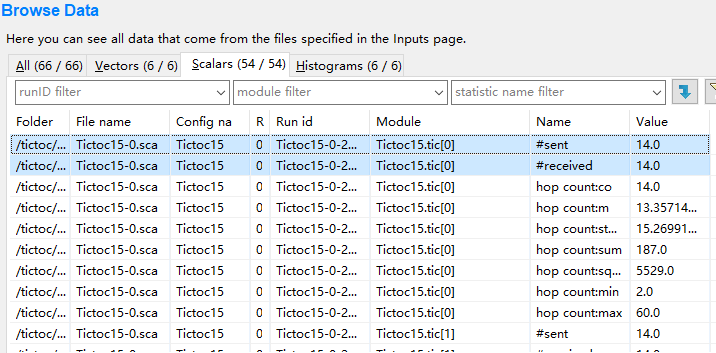
\includegraphics[keepaspectratio,width=\textwidth,height=0.75\textheight]{../img/chapter6/6-9.png}
\caption{doc目录}
\end{figure}

可以看到,如前文所述,文件名是匹配的

在Histogram栏中选中一条,并打开:

\begin{figure}[htbp]
\centering
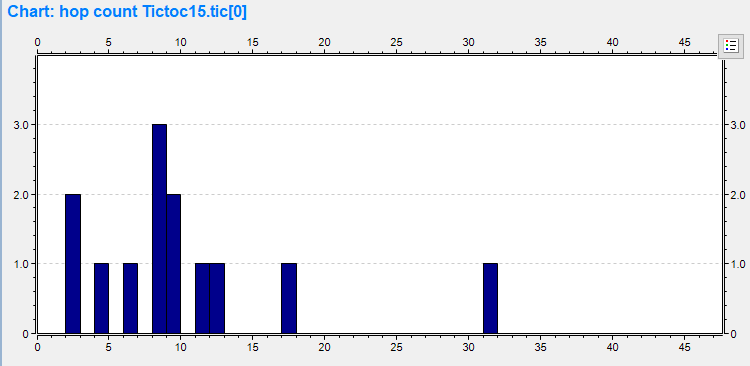
\includegraphics[keepaspectratio,width=\textwidth,height=0.75\textheight]{../img/chapter6/6-10.png}
\caption{doc目录}
\end{figure}

另外,我们也可以直接取出数据,方法如下:

\begin{figure}[htbp]
\centering
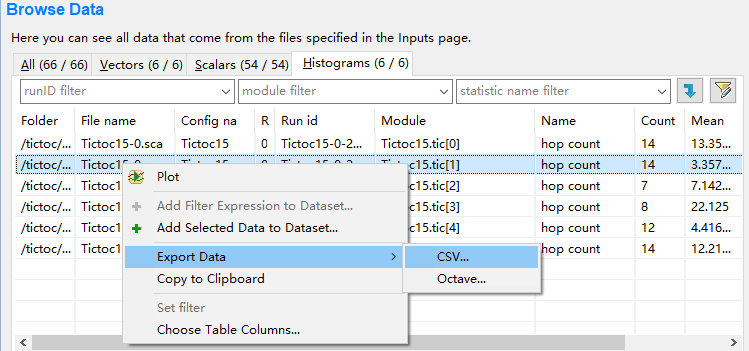
\includegraphics[keepaspectratio,width=\textwidth,height=0.75\textheight]{../img/chapter6/6-11.png}
\caption{doc目录}
\end{figure}

之后可以自己进行数据处理和作图。

\section{事件日志文件的使用}
\label{事件日志文件的使用}

事件日志文件(EventLog)所记录的内容包括用户仿真过程中各个模块发送的消息细节以及提示发送和消息接收的细节。在Tkenv界面进行仿真前,点击“Enable recording on\slash off”按钮,即可对仿真过程中的事件进行记录。

\begin{figure}[htbp]
\centering
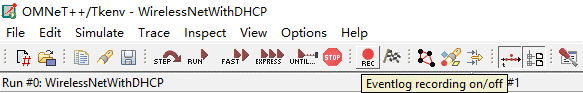
\includegraphics[keepaspectratio,width=\textwidth,height=0.75\textheight]{./../img/chapter6/6-12.png}
\caption{avatar}
\end{figure}

默认情况下,相应工程的result文件夹中会出现一个后缀为“.elog”的文件,即我们本次仿真记录所得的时间日志文件。这里需要特别注意的是,记录的数据数量会直接决定elog文件的大小,不仅会影响仿真的速度,还可能在仿真结束后,omnetpp无法打开过大的日志文件,导致闪退,严重时甚至出现过黑屏等情况。因此建议在使用时不要记录过长的时间或过多无用的内容。

\subsection{序列图}
\label{序列图}

打开elog文件后,里面的内容会以序列图的形式来展现,如下图所示:

\begin{figure}[htbp]
\centering
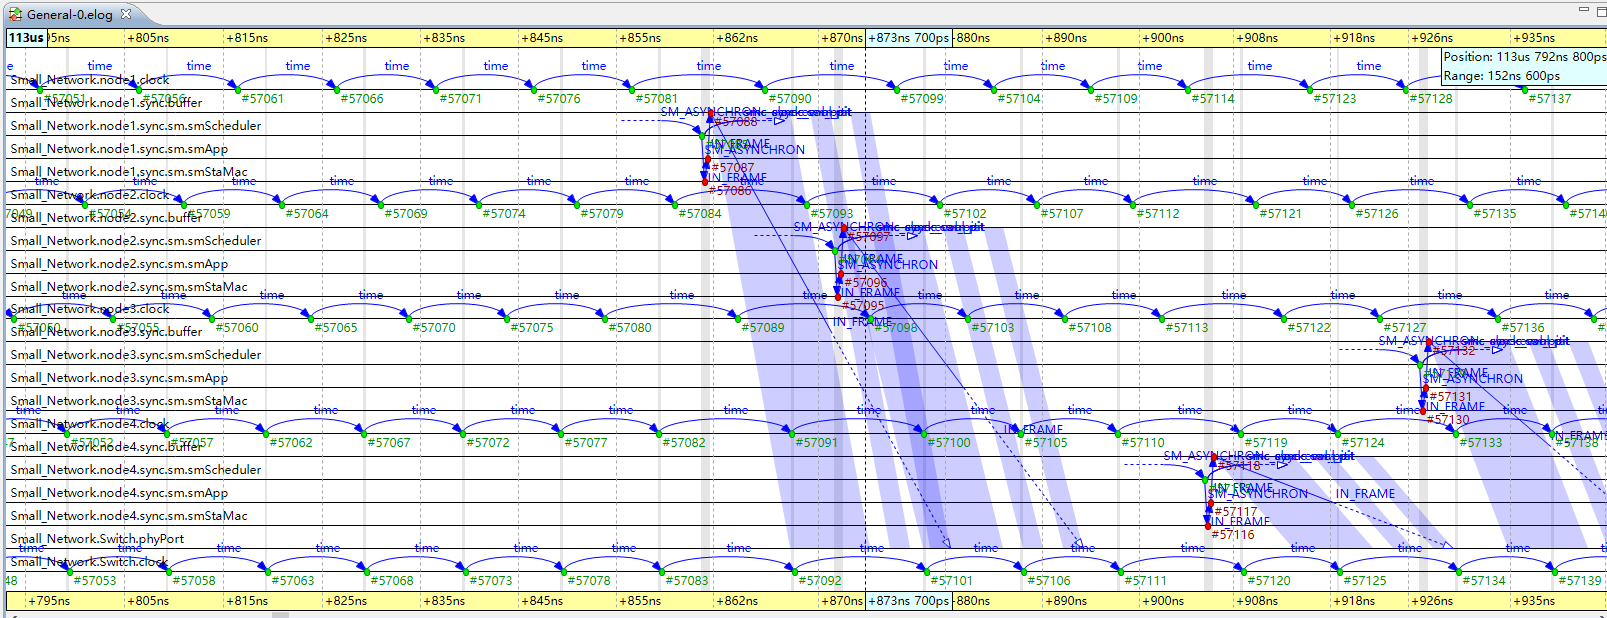
\includegraphics[keepaspectratio,width=\textwidth,height=0.75\textheight]{../img/chapter6/6-15.png}
\caption{常用符号}
\end{figure}

序列图可分为三个部分:上沿、主区域和下沿。其中,上下沿显示的是仿真时间轴。主区域则是显示各个模块名称和周线、时间与消息的发送。
下面是常用符号的图例:

\begin{figure}[htbp]
\centering
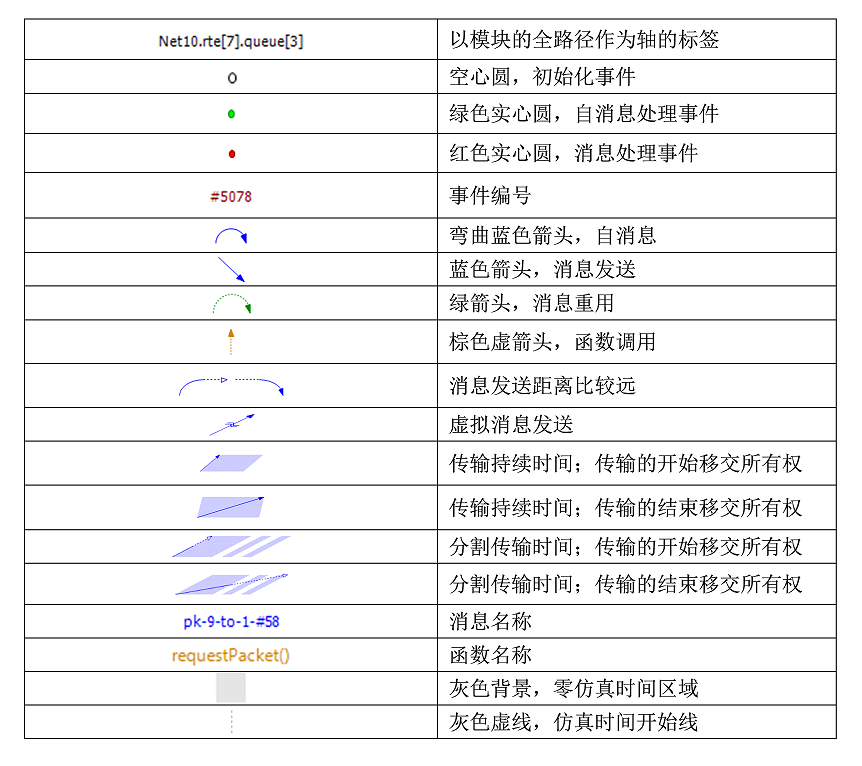
\includegraphics[keepaspectratio,width=\textwidth,height=0.75\textheight]{../img/chapter6/map_1.png}
\caption{常用符号}
\end{figure}

\subsection{事件日志表}
\label{事件日志表}

事件日志表的事件记录分为三栏,依次是事件编号、仿真时间和事件的具体细节。
善用过滤器来减少无用内容的显示对提高工作效率很有帮助,行过滤器可以过滤特定类型的显示行。同时,事件日志表支持导航历史纪录,每个用户停留超过三秒的位置都会被记录下来作为临时数据。

\begin{figure}[htbp]
\centering
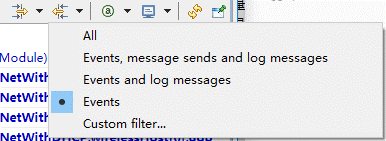
\includegraphics[keepaspectratio,width=\textwidth,height=0.75\textheight]{./../img/chapter6/6-13.png}
\caption{avatar}
\end{figure}

\subsection{个人体会}
\label{个人体会}

首先第一点,一定不要让elog文件的体积过大,因为这很可能导致处理过程中的闪退。
然后,过滤器是我最常用的功能。除了行过滤器外,序列图和事件日志表都支持同一个Filter。

\begin{figure}[htbp]
\centering
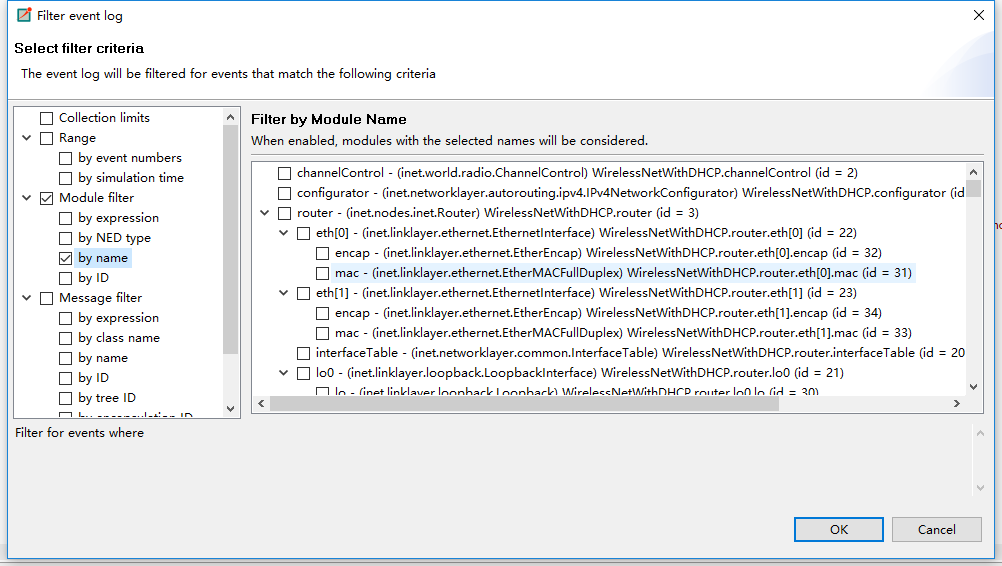
\includegraphics[keepaspectratio,width=\textwidth,height=0.75\textheight]{./../img/chapter6/6-14.png}
\caption{avatar}
\end{figure}

如图所示,一般包括:
范围过滤器:过滤掉elog中的起始和结束事件,有助于减少计算时间。
模块过滤器:用户可以指定特定的模块,非指定模块的事件会被全部过滤。当我们倾向于研究一个或几个特定模块时,这非常有用。
消息过滤器:最复杂的一个过滤器。需要根据消息的C++名称、消息名称、消息id以及匹配表达式等进行选择。
因果过滤器:通过指定特定的事件并对其愿意和结果进行过滤。

同时,omnet++对filter结果的计算和显示会耗费大量的时间,一定要指定适当的范围。具体根据什么来设置范围,就要以各位各自的使用情况作为标准了。

\chapter{错误记录}
\label{错误记录}

在我刚开始使用OMNeT++进行实验的时候,总是会出现一些稀奇古怪的错误,每一个错误都花了我大量的时间,所以在最后一章中总结出来,也许你正好用上。

\section{在模块加入移动模块之后,仿真出现nan错误}
\label{在模块加入移动模块之后,仿真出现nan错误}

\subsection{问题描述:}
\label{问题描述:}

\begin{quote}
对于某些工程加入移动模块以后,编译过程没有出错,但是当执行仿真程序的时候,出现一些nan错误提示。
需要在仿真配置文件加入:
\end{quote}

\begin{lstlisting}[language=c]
**.constraintAreaMinX = 0m
**.constraintAreaMinY = 0m
**.constraintAreaMinZ = 0m
**.constraintAreaMaxX = 5000m
**.constraintAreaMaxY = 5000m
**.constraintAreaMaxZ = 0m

\end{lstlisting}

移动模块配置:

\begin{lstlisting}[language=c]
**.UAV[*].mobilityType = "MassMobility"
**.UAV[*].mobility.initFromDisplayString = true
**.UAV[*].mobility.changeInterval = truncnormal(2s, 0.5s)
**.UAV[*].mobility.changeAngleBy = normal(0deg, 30deg)
**.UAV[*].mobility.speed = truncnormal(250mps, 20mps)
**.UAV[*].mobility.updateInterval = 100ms

\end{lstlisting}

\section{工程的例如cModule之类的类不能高亮显示?}
\label{工程的例如cmodule之类的类不能高亮显示?}

\subsection{问题描述}
\label{问题描述}

\begin{quote}
原工程是可以高亮显示的,但是由于我在备份这个程序的时候可能方式不对,我采用的是在文件资源管理器的窗口复制原工程文件夹,没有在软件的窗口进行rename,可能是这个原因造成的。
\end{quote}

\subsection{解决办法}
\label{解决办法}

在软件的窗口,对工程进行rename就行,编译一次,cMdoule等等关键词就可以高亮了。

\section{在建立工程时,需要实时显示节点的移动坐标时,编译出错}
\label{在建立工程时,需要实时显示节点的移动坐标时,编译出错}

\subsection{问题描述}
\label{问题描述}

\begin{quote}
在对节点的坐标进行实时的显示的过程中,编写如下的函数:
\end{quote}

\begin{lstlisting}[language=c]

void node::initialize()
{
    cModule *host = getContainingNode(this);
    IMobility *mobility = check_and_cast<IMobility *>(host->getSubmodule("mobility"));
    Coord selfPosition = mobility->getCurrentPosition();
}

\end{lstlisting}

同时以 ``inet\slash mobility\slash contract\slash IMobility.h''的形式引用头文件,但是在编译的过程中,会报出如下的错误:
..\slash out\slash clang-release\slash src\slash node.o:(.text{[\emph{ZN7omnetpp14check\_and\_castIPN4inet9IMobilityENS\_7cModuleEEET\_PT0}]}+0x18): undefined reference to \texttt{\_\_imp\_\_ZTIN4inet9IMobilityE'
..\slash out\slash clang-release\slash src\slash node.o:(.rdata[\_ZTIPN4inet9IMobilityE]+0x18): undefined reference to}typeinfo for inet::IMobility'

\subsection{解决办法:}
\label{解决办法:}

方法一:
在inet中将IMobility.h中第一行将 ``INet\_API'' 删除后,重新对inet进行编译,然后在对所建立的工程进行编译,编译既可以通过。
方法二:
打开当初安装OMNET++ 的文件夹,找到configure.user的文本,打开后,找到CC==gcc,将前面的“\#”注释符号去掉;然后打开mingwenv.cmd
,按顺序先后执行``.\slash configure'' and ``make''命令,编译完成后,重新对工程进行编译即可。

\section{在进行移动模型的构建时,如何可以看到移动轨迹}
\label{在进行移动模型的构建时,如何可以看到移动轨迹}

\subsection{问题描述}
\label{问题描述}

当节点进行移动的时候,想观察节点的移动轨迹,那么如何进行操作?

\subsection{解决办法:}
\label{解决办法:}

完成这个问题,需要进行两步操作,分别在.ned .ini文件中:
1)在整个网络拓扑ned文件中,需要添加必要的路径和模块:

\begin{lstlisting}[language=c]
/*调用inet中的库函数*/
import inet.visualizer.integrated.IntegratedCanvasVisualizer;
import inet.visualizer.contract.IIntegratedVisualizer;

//添加visualizer模块
visualizer: <default("IntegratedCanvasVisualizer")> like IIntegratedVisualizer if hasVisualizer() {
    parameters:
        @display("p=50103.34,27751.85");
}
\end{lstlisting}

2)然后在.ini文件中进行配置

\begin{lstlisting}[language=c]

*.visualizertype = "IntegratedOsgVisualizer"
*.hasVisualizer = true
*.visualizer.mobilityVisualizer.moduleFilter = "**"
*.visualizer.mobilityVisualizer.displayMovementTrails = true
*.visualizer.mobilityVisualizer.movementTrailLineColor = "dark"
*.visualizer.mobilityVisualizer.movementTrailLineStyle = "solid"
*.visualizer.mobilityVisualizer.movementTrailLineWidth =  2
*.visualizer.mobilityVisualizer.trailLength = 100000
*.visualizer.mobilityVisualizer.displayOrientations = true
*.visualizer.mobilityVisualizer.displayVelocities = true

\end{lstlisting}

通过以上两步就可以实现完成轨迹的显示

\chapter{TODO 待完善}
\label{todo待完善}

\begin{itemize}
\item {[1]} 如何加快节点间消息的传输?

\item {[2]} 在一个复合模块下,如何访问同一级的其他模块?

\item {[3]} 如何得到某一个模块引用的ned路径?

\item {[4]} 如何使用cTopology类遍历网络的拓扑来初始化路由表?

\item {[5]} 如何在omnet上使用OpenSceneGraph

\item {[6]} 如何从仿真场景读取节点的坐标

\item {[7]} 使用sendDirect()函数

\item {[8]} 复合模块初始化时,先初始化节点的顺序

\item {[9]} 在initialize()中初始化类成员数组与在其他函数中的不同

\end{itemize}

\appendices
\renewcommand{\prechap}{\appendixname}
\renewcommand{\postchap}{}
%appendix
\chapter{网络性能指标}
\label{网络性能指标}

\&\#160; \&\#160; \&\#160; \&\#160;在前面几章中总是会涉及到相关网络中的术语,可能不利于读者理解,因此在最后加上附录,完善相关内容。

\section{1 速率}
\label{1速率}

\&\#160; \&\#160; \&\#160; \&\#160;主要是指主机在数字通信上传送数据的速率,称为额定速率或者标称速率。
定义:单位时间(秒)传输信息量(比特)通常情况下用bit符号表示。
常用的单位:b\slash s, kb\slash s, Mb\slash s, Gb\slash s,他们之间的换算关系为:
$$1Gb/s = 10^6 Mb/s = 10^9 b/s$$

\section{2 吞吐率}
\label{2吞吐率}

\&\#160; \&\#160; \&\#160; \&\#160;网络通信中发送端与接收端之间传送数据的速率。吞吐量受到网络的带宽或网络的额定速率的限制。

\begin{itemize}
\item 即时吞吐率:给定时刻的速率;

\item 平均吞吐率:一段时间的平均速率;

\item 瓶颈链路:端到端路劲上,带宽最小的链路。

\end{itemize}

\&\#160; \&\#160; \&\#160; \&\#160;吞吐率决定瓶颈链路的带宽,吞吐率为发送端的发送速率, 发送端发送数据的速率大于瓶颈链路,则吞吐率为瓶颈链路的带宽。

\section{3 延迟}
\label{3延迟}

\&\#160; \&\#160; \&\#160; \&\#160;数据在传输过程中所消耗的时间即称为延迟,在分组交换网络中,延迟总共包含有四种:即节点处理延迟、排队延迟、传输延迟、传播延迟。

\begin{itemize}
\item {[1]} 节点处理延迟
节点(路由器)在处理数据时进行差错检测、确定链路输出等活动小号的时间,通常时间延迟很小,一般为毫秒级甚至更低。

\item {[2]} 排队延迟
需要传输的数据在节点中等待输出链路可用所花的时间,往往取决于节点(路由器)的拥塞程度。

\item {[3]} 传输延迟
节点将正在传输的分组数据发送到输出链路所用的时间,取决于L:分组长度(bit)和R:链路带宽,延迟d=L\slash R;

\item {[4]} 传播延迟
信号在信道中传播所用的时间,取决于信道长度d和电磁波信号在信道上的传播速度,延迟Pd=d\slash s

\item {[5]} 总时延
将上述的四个时延时间进行相加,既可以得到。

\end{itemize}

\section{4 丢包率}
\label{4丢包率}

\&\#160; \&\#160; \&\#160; \&\#160;丢包数\slash 已发分组的总数,分组交换网络丢包的原因主要是节点的队列缓存容量有限,当分组到达时如果节点中的分组队列已满,则该分组会被丢弃,即称为丢包。

\section{5 带宽}
\label{5带宽}

\begin{itemize}
\item 信号的带宽
信号的带宽是指信号所包含的各种不同频率成分所占据的频率范围。

\item 计算机网络的带宽
在单位时间内从网络中的某一点到另一点所能通过的最高数据率,即网络可通过的最高数据率,即每秒传输多少比特,单位是“比特每秒”,或b\slash s(bit\slash s)。

\end{itemize}

\section{6 时延带宽积}
\label{6时延带宽积}

\&\#160; \&\#160; \&\#160; \&\#160;将两个网络性能的两个度量,传播时延和宽带相乘,就等到另外一个度量:传播时延带宽积(单位:bit;)。
$$时延带宽积=传播时延*带宽$$

\&\#160; \&\#160; \&\#160; \&\#160;下面是一个简单的例子:传播时延为20ms,带宽为10Mb\slash s,则时延带宽积 = 20 × 10 × 10\textsuperscript{3} \slash 1000 = 2 × 10\textsuperscript{5} bit。这就表示,若发送端连续发送数据,则在发送的第一个比特即将达到终点时,发送端就已经发送了20万个比特,而这20万个bit都在链路上向前移动。

\section{7 信道利用率}
\label{7信道利用率}

\&\#160; \&\#160; \&\#160; \&\#160;信道利用率是指信道有百分之几的时间是被占用的比率,其计算公式如下:
$$S=发送时间T /(传播时延t+碰撞等待时间2n*t+发送时间)$$

\&\#160; \&\#160; \&\#160; \&\#160;上述提到的发送时间T是指:T=帧长数\slash 发送速率。
这里有一个简单例子加以说明,假设信道的长度为10km,往返传输时延为10ms,传输数据长度为2048bit,发送端的发送速率为1Mbps,在其他时延(碰撞等待时间)忽略的情况下,求信道利用率。

\begin{itemize}
\item 发送时间:2048\slash (1x1000x1000)=2.048ms

\item 信道利用率:2.048\slash (2.048+10)=17\%

\end{itemize}

\section{9 网络利用率}
\label{9网络利用率}

\&\#160; \&\#160; \&\#160; \&\#160;网络利用率是指全网络的信道利用率的加权平均值。

\section{10 往返时间RTT}
\label{10往返时间rtt}

\&\#160; \&\#160; \&\#160; \&\#160;表示从发送方发送数据开始,到发送方收到来自接收方的确认,总共经历的时间。
其与所发送的分组长度有关。发送很长的数据块的往返时间,应当比发送很短的数据块往返时间要多。

\end{document}
